% Preamble
\documentclass[12pt]{report}
\usepackage[utf8]{inputenc}
\usepackage{graphicx}
\usepackage{amsmath}
\usepackage{amsfonts}
\usepackage{nicematrix}


\graphicspath{ {images/} }

\usepackage[a4paper,width=150mm,top=20mm,bottom=20mm,bindingoffset=6mm]{geometry}

\usepackage{fancyhdr}
\pagestyle{fancy}
\fancyhead{}
\fancyhead[RO,LE]{Implementing Fast Multipole Methods with High-Level Interpreted Languages}
\fancyfoot{}
\fancyfoot[LE,RO]{\thepage}
\fancyfoot[LO,CE]{Chapter \thechapter}
\fancyfoot[CO,RE]{Srinath Kailasa}

\usepackage{titlesec}

\titleformat{\chapter}[display]
  {\normalfont\bfseries}{}{0pt}{\Huge}

\usepackage[backend=bibtex]{biblatex}
\addbibresource{references.bib}


\usepackage{lipsum}
\usepackage[toc]{glossaries}

\makeglossaries
\newglossaryentry{latex}
{
    name=latex,
    description={Is a mark up language specially suited
    for scientific documents}
}

\newglossaryentry{far-field}{
    name={far field},
    description={
        An set of particles in the far field are considered to be far away enough
        from the particle of interest that they are suitably described by a
        convergent multipole expansion.
    }
}

\newglossaryentry{near-field}{
    name={near field},
    description={
        An set of particles in the near-field are considered to violate the
        the criteria for describing them with a convergence multipole expansion.
    }
}

\newglossaryentry{near-neighbours}
{
    name={near neighbours},
    description={
        Two boxes in computational tree are near neighbours if they are at the
        same level of refinement, and share a boundary point.
    }
}

\newglossaryentry{well-separated}
{
    name={well separated},
    description={
        Two boxes in computational tree are near neighbours if they are at the
        same level of refinement, and are not near neighbours.
    }
}

\newglossaryentry{interaction-list}{
    name={interaction list},
    description={
    Boxes which are the children of the near-neighbours of the a box's
    parent box, but are not adjacent to the box itself.
    }
}

\newglossaryentry{FMM}{
    name={FMM},
    description={
        The Fast Multipole Method.
    }
}

\newglossaryentry{KIFMM}{
    name={KIFMM},
    description={
        The `Kernel Independent' Fast Multipole Method.
    }
}

\newglossaryentry{post-order}{
    name={post-order},
    description={
        In reference to the traversal of heirarchical trees, post-order traversal
        is moving from the finest (leaf) level to the coarsest (root) level.
    }
}

\newglossaryentry{pre-order}{
    name={pre-order},
    description={
        In reference to the traversal of heirarchical trees, pre-order traversal
        is moving from the coarsest (root) level to the finest (leaf) level.
    }
}

\newglossaryentry{P2M}{
    name={P2M},
    description={Particle to multipole expasion operation.}
}

\newglossaryentry{M2M}{
    name={M2M},
    description={Translate from multipole of child box to multipole expansion
    of parent box.}
}

\newglossaryentry{M2L}{
    name={M2L},
    description={Translate from multipole of box $A$ to local expansion
    of box $B$.}
}

\newglossaryentry{L2L}{
    name={L2L},
    description={Translate from local of parent box to local expansion
    of child box.}
}

\newglossaryentry{L2P}{
    name={L2P},
    description={Evaluate local of leaf box at each target particle in a leaf
    box.}
}

\newglossaryentry{P2P}{
    name={P2P},
    description={
        Evaluate particle to particle interactions directly.
    }
}

\newglossaryentry{target-particles}{
    name={target particles},
    description={
        Particles are described as targets if the potential due to a source field
        is being evaluated at these particle's positions, but they themselves are
        not being considered as a source for the field being evaluated. They may
        or may not refer to the same set of particles as the source particles,
        for example in the classic $N$-Body problem, the target particles and
        the source particles are the same set.
    }
}

\newglossaryentry{source-particles}{
    name={source particles},
    description={
        Particles are described as sources if they are consifered to contribute
        to the source field being evaluated at the target particles. They may
        or may not refer to the same set of particles as the target particles,
        for example in the classic $N$-Body problem, the target particles and
        the source particles are the same set.
    }
}

\newglossaryentry{task-level-parallelism}{
    name={task-level parallelism},
    description={
        Task-level parallelism is achieved when multiple threads or processes,
        running the same, or differing, code, in a multiprocessing system are
        executed with the same, or differing, data.
    }
}

\newglossaryentry{instruction-level-parallelism}{
    name={instruction-level-parallelism},
    description={
        Instruction-level parallelism refers to the parallel execution of different
        instructions on a specific thread or process in a multiprocessing system.
    }
}

\newglossaryentry{data-level-parallelism}{
    name={data-level parallelism},
    description={
        In a multiprocessor system, data level parallelism is achieved by
        distributing data amongst different compute nodes to be executed upon
        in parallel. See \textbf{CUDA}
    }
}

\newglossaryentry{CUDA}{
    name={CUDA},
    description={
        `Compute Unified Device Architecture', is a parallel computing API
        designed for the development of programs for \textbf{GPU}s
    }
}

\newglossaryentry{GPU}{
    name={GPU},
    description={
        `Graphics Processing Unit', are specialised processors specifically
        designed for rapid parallel execution across large blocks of data.
    }
}

\newglossaryentry{SIMD}{
    name={SIMD},
    description={
        Single Instruction, Multiple Data.
    }
}

\newglossaryentry{high-level-interpreted-language}{
    name={high level interpreted language},
    description={
        A High-Level language is one that offers an API and primitive data
        structures that strongly abstract from the details of the computer on
        which it is being run. An interpreted language is one in which codes
        are run directly via an \textit{interpreter}, rather than first being
        compiled. In reality interpreted languages run in a `virtual machine',
        which takes input code, transforms it to byte-code which is then translated
        into machine level instructions. This approach allows for greater portability
        of code, and developer productivity, at the expense of space and time overhead
        in running software.
    }
}

\newglossaryentry{source-densities}{
    name={source densities},
    description={
        Source densities are associated with their respective \textbf{source particles}.
        In electromagnetic problems, these would correspond to charges. In gravitational
        problems, these would correspond to mass.
    }
}

\newglossaryentry{equivalent-density}{
    name={equivalent density},
    description={
        An equivalent representation of the potential generated by a discrete/continuous
        distribution. This equivalent density is supported at discrete points on
        an \textbf{equivalent surface}.
    }
}

\newglossaryentry{equivalent-surface}{
    name={equivalent surface},
    description={
        An equivalent surface supports equivalent density points.
    }
}

\newglossaryentry{check-surface}{
    name={check surface},
    description={
        Defines the surface at which the potential caused by source points, and
        the equivalent density formulation coincide.
    }
}

\newglossaryentry{check-potential}{
    name={check potential},
    description={
        The potential calculated from source particles, or an equivalent density
        distribution at a check surface.
    }
}

\newglossaryentry{PDE}{
    name={PDE},
    description={
        Partial Differential Equation.
    }
}

\newglossaryentry{SVD}{
    name={SVD},
    description={
        Singular Value Decomposition.
    }
}

\newglossaryentry{FFT}{
    name={FFT},
    description={
        Fast Fourier Transform.
    }
}

\newglossaryentry{MPI}{
    name={MPI},
    description={
        Message Passing Interface for implementing distributed memory parallelism.
        Each process is given it's own local memory, and can communicate and pass
        data and computational results to other processes being run in parallel.
    }
}

\newglossaryentry{OpenMP}{
    name={OpenMP},
    description={
        Open MultiProcessing is an API for implementing shared-memory parallelism.
        Each process is run on a separate thread, but a global memory space is
        shared.
    }
}

\newglossaryentry{PyExaFMM}{
    name={PyExaFMM},
    description={
        The Python implementation of the \textbf{KIFMM} presented as a part of this
        thesis.
    }
}

\newglossaryentry{object-oriented-language}{
    name={Object Oriented Language},
    description={
        Programming paradigm in which data and methods are abstracted into
        `objects'. This allows for the separation of data and logic into
        structures that encapsulate their logical grouping.
    }
}

\newglossaryentry{interpreted}{
    name={interpreted},
    description={
        In reference to an interpreted programming language. Here instead of
        direct compilation of source code into machine level instructions, source
        code is passed to an `interpreter', which compiles a byte-code on the programmers
        behalf. This byte-code is sent to a compiler as it arrives, giving the programmer
        the illusion of interactive programming.
    }
}

\newglossaryentry{JIT}{
    name={JIT},
    description={
        Just-In-Time compilation ...
    }
}

\newglossaryentry{key}{
    name={key},
    description={
        In the context of space filling curves, refers to the encoded position
        along the length of a curve.
    }
}

% Default fixed font does not support bold face
\DeclareFixedFont{\ttb}{T1}{txtt}{bx}{n}{12} % for bold
\DeclareFixedFont{\ttm}{T1}{txtt}{m}{n}{12}  % for normal

% Custom colors
\usepackage{color}
\definecolor{deepblue}{rgb}{0,0,0.5}
\definecolor{deepred}{rgb}{0.6,0,0}
\definecolor{deepgreen}{rgb}{0,0.5,0}

\usepackage{listings}

% Python style for highlighting
\newcommand\pythonstyle{\lstset{
language=Python,
basicstyle=\ttm,
otherkeywords={self},             % Add keywords here
keywordstyle=\ttb\color{deepblue},
emph={MyClass,__init__},          % Custom highlighting
emphstyle=\ttb\color{deepred},    % Custom highlighting style
stringstyle=\color{deepgreen},
frame=tb,                         % Any extra options here
showstringspaces=false            %
}}


% Python environment
\lstnewenvironment{python}[1][]
{
\pythonstyle
\lstset{#1}
}
{}

% Python for external files
\newcommand\pythonexternal[2][]{{
\pythonstyle
\lstinputlisting[#1]{#2}}}

% Python for inline
\newcommand\pythoninline[1]{{\pythonstyle\lstinline!#1!}}

\begin{document}


    \begin{titlepage}
    \begin{center}
        \vspace*{1cm}
        
        \Huge
        \textbf{Accellerating Fast Multipole Methods}
        
        \Large
        \vspace{0.5cm}
        subtitle
             
        \vfill
 
        \textbf{Srinath Kailasa}
 
        \vspace{5cm}
             
        A thesis presented for the degree of\\
        Master of Science
             
        \vspace{0.8cm}
      
        
\includegraphics[width=0.4\textwidth]{university.png}
        
        \large
        Department of Physics\\
        University College London\\
        \today
             
    \end{center}
 \end{titlepage}

    \thispagestyle{plain}

\begin{center}
    \textbf{Declaration}
\end{center}
I, Srinath Kailasa, confirm that the work presented in this thesis is my own. Where information has been derived from other
sources, I confirm that this has been indicated in the thesis.


\begin{center}
    \textbf{Acknowledgements}
\end{center}

This thesis has been the product of two very long and concurrently short years
at UCL. Returning to education whilst extricating myself from industry presented a set
of challenges which I wasn't entirely expecting, but thrilled to have overcome. I'd
like to thank my Mum for keeping me on the right path, and without whose support
this thesis would probably never have happened. Furthermore, I'd like to thank my
supervisor Timo Betcke, whose door was always open, I couldn't really have asked
for a much better thesis supervisor; and with whom, Master's in hand, I'm greatly
looking forward to starting my PhD with in the autumn.


    \newpage

    \thispagestyle{plain}

\begin{center}
    \textbf{Declaration}
\end{center}
I, Srinath Kailasa, confirm that the work presented in this thesis is my own. Where information has been derived from other
sources, I confirm that this has been indicated in the thesis.

\begin{center}
    \textbf{Abstract}
\end{center}

The Fast Multipole Method (FMM) is a numerical approach to accelerating the solution
of the `n-body' problem, which appears in numerous situations in science and engineering,
for example in solving for gravitational or electrostatic potentials. It does so by approximating
the Green's function of the
system with analytic infinite series expansions (the origin of the `multipole' in its name),
 and coalescing the effect of distinct distant sources together so as to
reduce the number of computations. The analytic expansions of the
original Fast Multipole Method depend on the Green's function of the system in
question (Helmholtz, Laplace etc.), and in practice a new implementations
must be written for a given system.

The Kernel Independent Fast Multipole Method (KIFMM),
first presented by Ying et al. \cite{ying}, is a similar approach that replaces
the analytic series expansions with a continuous distribution of so called
`equivalent density' supported at discrete points on a box enclosing a set of
particles. These equivalent densities are found by matching the potential they
generate to those generated by the original sources at another surface in the
far field. Usefully, this approach doesn't require multipole expansions of the
Green's functions of a system, and therefore can be programmed in an agnostic way,
hence the origin of it's name.

This thesis presents a Python implementation of
the KIFMM, with investigations made into both mathematical and computational
techniques for the acceleration of the algorithm. Python is chosen as it has emerged as a standard
for scientific and data intensive computing in recent years, with a huge increase
in usage and a well supported ecosystem of libraries and tools available for
accelerating numerical codes. The wider context of this thesis
is an ongoing collaboration with the ExaFMM Project \cite{exafmm} to produce a Pythonic
implementation of the KIFMM that can compete in terms of performance with
a C++ equivalent. This thesis presents a systematic performance analysis
of a naive implementation of the KIFMM algorithm, before proceeding to examine and implement
acceleration techniques. The speed and accuracy of the implementation is tested
for some simple Green's functions, and it concludes with a discussion on future avenues
for investigation.

    \tableofcontents

    \chapter{Introduction}\label{chapter:introduction}
\section{Overview of the Analytic FMM}
\subsection{Motivation}
The paradigmatic problem of Fast Multipole Methods (\textbf{\gls{FMM}})
\footnote{The first usage of a technical term or abbreviation listed in the
glossary is highlighted throughout the text for ease of reference.} is the so
called $N$-Body problem. This classic problem refers to the calculation of the pairwise
interactions between $N$ particles over a potentially long-range, for example in
gravitational or electrostatic problems. The straightforward calculation can be
written in the form of the following sum,

\begin{equation}
\Phi(x_j) = \sum_{i=1}^N w_i K(x_i, x_j)
\label{eq:n_body_problem}
\end{equation}

Where $i, j \in [1,N]$ and $K(x, y)$ is called the Green's function, or equivalently
a `kernel function', where one is generally concerned with coordinates of particles in an
$n=2 \> \> \text{or} \> \> 3$ dimensional Hilbert space taking  $\ x_i \in \mathbb{R}^n$.
Additionally, each summand is weighted by $w_i$. For solving for electrostatic
potential in three dimensions, which is used as the model problem throughout this
thesis, this goes to,

\begin{equation}
\Phi(x_j) = \sum_{i=1}^N q_iK(x_i, x_j)
\label{eq:electrostatic_paradigm}
\end{equation}

where $q_i$ refers to a charge density with the kernel function,

\begin{equation}
    K(x, y) = \frac{1}{4\pi \epsilon_0}\frac{1}{| x - y |}
\label{eq:laplace_kernel}
\end{equation}

the constant $\epsilon_0$ is the permittivity of free space. For practical
purposes, we define $K(x,x) = 0$. It's easy to see
how a naive direct application of this equation over $N$ particles
results in an algorithm of $O(N^2)$ complexity, therefore it's only practicable
for systems of moderate size, whereas in realistic systems, one may be interested in
interactions involving $10^{6}$ to $10^8$ particles.

This chapter introduces the analytic \gls{FMM}, the kernel-independent
version, which is the main focus of this thesis, is presented later.
Though substantially different in implementation, the analytic FMM will provide the opportunity
to exposit many of the key ideas behind all FMM-based algorithms, and provides
a good starting point for understanding and developing upon these algorithms.
First presented by Greengard \cite{Greengard:1987:JCP},
the analytic \gls{FMM} represented a sea change for $N$-Body simulation. By
trading off computations for error, it manages to achieve an asymptotic complexity
 of just $O(N)$. Additionally, it comes equipped with rigorous error bounds,
making fast and accurate massive $N$-Body simulations feasible on available
computing hardware. It's success has been such that it is regarded as one of
the key developments in numerical algorithms in the twentieth century \cite{Cipra:2000:SN}.

The original analytic FMM solves the electrostatic problem
in two and three dimensions, this is equivalently known as the Poisson problem,
represented by the differential equation,

\begin{equation}
    \nabla^2 \phi =f
\label{eq:poisson}
\end{equation}

Where $\phi$ is some scalar potential to be determined, and $f$ is a scalar source
term which is usually known. For electrostatics the corresponding formulation
can be derived from Gauss' law as \cite{Griffiths:2017:CUP},

\begin{equation}
  \nabla^2 \phi = - \frac{q}{\epsilon_0}
\label{eq:electrostatic_poisson}
\end{equation}

where $\phi$ is the electrostatic potential, $q$ is the charge density and
$\epsilon_0$ is the permittivity of free space. It can therefore be seen that
the \gls{FMM} is actually solving the Poisson problem by reformulating it as an
integral equation \cite{Epton:1995:SIAM}. The ubiquity of problems of the form (\ref{eq:n_body_problem})
in computational science has lead to diverse application of the FMM. For example,
in the modeling the electrostatic interactions of charged particles in complex
biological molecules at biologically relevant length scales \cite{Board:1992:CPL}.
The extension of FMMs to Helmholtz equations \cite{Rokhlin:1990:JCP}, has lead
to even more applications, such as in seismic and acoustic scattering
\cite{Hwu:2011:MKP}. Though as the focus of this thesis is on solving the Poisson
model problem for electrostatics, this is mentioned only for completeness.

The key insight that leads to the \gls{FMM}'s asymptotic complexity is the idea
that if the field created by a distribution of charge (or mass) density is approximated
to be relatively smooth in the \textbf{\gls{far-field}}, then it should be possible to apply
some form of compression for the evaluation of contribution to local potentials due
to particles in the \gls{far-field}. The FMM performs this compression by encoding
the field contributions of particles in the \gls{far-field} using a multipole
expansion.

For simple kernel functions and charge distributions, such as the model problem
of this thesis, one can easily derive the expression for this multipole expansion
by finding an series expansion of the system's Green's function.
In order to generalise the discussion, an arbitrary continuous
distribution of charge is considered as shown in figure \ref{fig:1_1_continuous_charge_distribution},
for which the potential is evaluated at some other evaluation point outside of
the distribution. This can be written as follows \cite{Griffiths:2017:CUP},

\begin{flalign}
    \Phi(\mathbf{r}) = \frac{1}{4 \pi \epsilon_0} \int \frac{1}{d}\rho(\mathbf{r}')d\tau'
    \label{eq:1_1_continuous_integral_formulation}
\end{flalign}

where $\rho(\mathbf{r}')$ is a charge density, and the other symbols take their
meanings from figure (\ref{fig:1_1_continuous_charge_distribution}).


\begin{figure}[!h]
    \centering
    {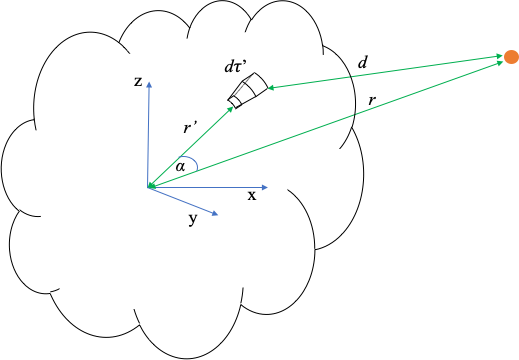
\includegraphics[width=0.45\textwidth]{introduction/continuous_charge.png}}
  \vspace{0pt}
  \caption{An arbitrary charge distribution, with an orange point to mark a point
  where the potential is being evaluated. Here, $\mathbf{r}$ is the the vector
  between the centre of the multipole expansion and the evaluation point, $\mathbf{r}'$
  is the vector between the centre of expansion and a given volume element $d\tau'$, and
  $d$ is a vector between the volume element $d\tau'$ and the evaluation point.}
  \label{fig:1_1_continuous_charge_distribution}
\end{figure}

From law of the cosines,

\begin{flalign}
    d^2 &= r^2 + (r')^2 - 2rr'\cos \alpha = r^2 \left [ 1 + \left ( \frac{r'}{r} \right)^2 - 2 \left (\frac{r'}{r} \right)\cos \alpha \right]\\
    d &= r \sqrt{1+\epsilon},
    \label{eq:1_1_law_of_cosines}
\end{flalign}

where,

\begin{flalign}
    \epsilon \equiv \left ( \frac{r'}{r} \right) \left (\frac{r'}{r} - 2 \cos \alpha \right)
\end{flalign}

As $\epsilon$ is small far away from charge distribution one can expand $1/d$ binomially,

\begin{flalign}
    \frac{1}{d} &= \frac{1}{r}(1+\epsilon)^{-1/2} = \frac{1}{r}\left (1 - \frac{1}{2}\epsilon + \frac{3}{8}\epsilon^2 - ... \right) \\
    \frac{1}{d} &= \frac{1}{r} \sum_{n=0}^{\infty} \left(\frac{r'}{r} \right)^n P_n(\cos \alpha)
\end{flalign}

Using this, the exact multipole expansion for this charge distribution is,

\begin{flalign}
    \Phi(\mathbf{r}) = \frac{1}{4 \pi \epsilon_0}\sum_{n=0}^{\infty}\frac{1}{r^{n+1}}\int (r')^nP_n(\cos \alpha)\rho(\mathbf{r'}) d \tau'
\end{flalign}

If instead one considers a charge distribution composed of $N$ discrete charges
$q_i$ at positions $r_i$, this goes to,

\begin{flalign}
    \Phi(\mathbf{r}) = \frac{1}{4 \pi \epsilon_0}\sum_{i=1}^N\sum_{n=0}^{\infty}\frac{(r_i)^n q_i}{r^{n+1}}P_n(\cos \alpha)
\end{flalign}

Using the addition theorem for Legendre polynomials \cite{Greengard:1987:Yale},

\begin{flalign}
    P_n(\cos \gamma) = \sum_{m=-n}^n Y_n^{-m}(\alpha, \beta) Y_n^m(\theta, \phi),
\end{flalign}

where the Legendre polynomial is written in terms of spherical harmonics,
where $(r, \theta, \phi)$ and $(\rho, \alpha, \beta)$ define two spherical coordinates,
and $\gamma$ is the angle subtended between them. Therefore, the multipole expansion goes to,

\begin{flalign}
    \Phi(\mathbf{r}) &= \frac{1}{4 \pi \epsilon_0}\sum_{i=1}^N\sum_{n=0}^{\infty}\frac{(r_i)^n q_i}{r^{n+1}}P_n(\cos \alpha)\\
    & = \frac{1}{4 \pi \epsilon_0}\sum_{i=1}^N\sum_{n=0}^{\infty}\sum_{m=-n}^n \frac{(r_i)^n q_i Y_n^{-m}(\alpha_i, \beta_i) }{r^{n+1}}Y_n^m(\theta, \phi)\\
    & = \frac{1}{4 \pi \epsilon_0}\sum_{n=0}^{\infty}\sum_{m=-n}^n M_n^m \cdot \frac{Y_n^m(\theta, \phi)}{r^{n+1}}  ,
    \label{eq:1_1_multipole_expansion}
\end{flalign}

where,

\begin{equation}
    M_n^m = \sum_{i=1}^N (r_i)^n q_i Y_n^{-m}(\alpha_i, \beta_i)
\end{equation}

This is an exact expansion, and it converges for $\frac{r_i}{r} < 1$. This convergence
condition means that estimating of the potential at a given evaluation point
calculated using the multipole expansion is only possible in the far-field, the
boundary of which is often tuned empirically for different systems as it's user
defined. If instead the expansion is taken with centre at the evaluation point,
one can rewrite as the multipole expansion as a `local' expansion,

\begin{flalign}
    \Phi(\mathbf{r}) & = \frac{1}{4 \pi \epsilon_0}\sum_{i=1}^N\sum_{n=0}^{\infty}\sum_{m=-n}^n \frac{(r)^n q_i Y_n^{-m}(\alpha_i, \beta_i) }{(r_i)^{n+1}}Y_n^m(\theta, \phi)\\
    & = \frac{1}{4 \pi \epsilon_0} \sum_{n=0}^{\infty} \sum_{m=-n}^n L_n^m \cdot  Y_n^m(\theta, \phi) \cdot r^n,
    \label{eq:1_1_local_expansion}
\end{flalign}

where,

\begin{equation}
    L^m_n = \sum_{i=1}^N \frac{q_i Y^{-m}_n(\alpha_i, \beta_i)}{(r_i)^{n+1}},
\end{equation}

which converges when $\frac{r}{r_i} < 1$. The region of convergence for both types
of expansions are shown in figure (\ref{fig:1_1_multipole_local_expansions}).

The key point to note is that the multipole and local expansions are exact, and
can be truncated as required to ensure that the asymptotic complexity of evaluating
a multipole or local expansion at an evaluation point is bounded by $O(N)$. A
rigorous error analysis of the analytic FMM is outside the scope of this thesis, and
we defer to the literature for exact expressions for these truncation errors \cite{Greengard:1987:Yale},
Furthermore, exact operations exist for shifting the center of these expansions,
as well as translating multipole expansion coefficients into equivalent local expansion
coefficients,
which are crucial in providing the improvements to asymptotic complexity\footnote{
    Expressions for these shift operators for the three dimensional Laplace kernel
    considered as our model problem are provided in Appendix \ref{app:3d_laplace}.
}.

\begin{figure}[!h]
    \centering
    {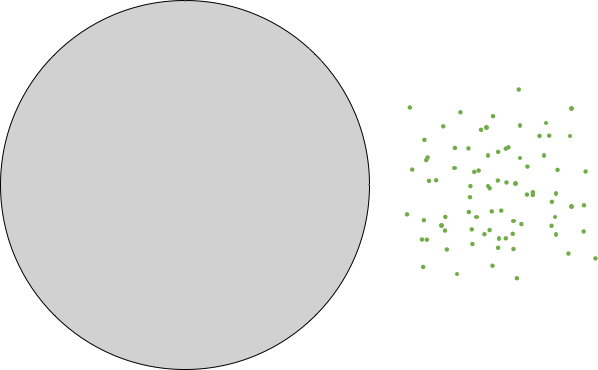
\includegraphics[width=0.33\textwidth]{introduction/multipole_expansion.png}}
    \hfill
  {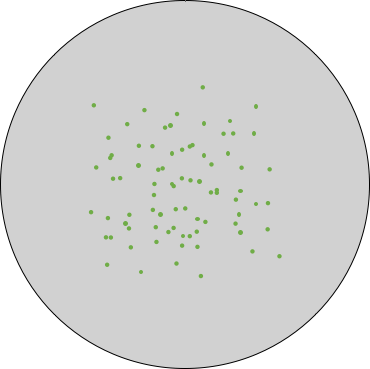
\includegraphics[width=0.4\textwidth]{introduction/local_expansion.png}}
  \vspace{0pt}
  \caption{(A) A multipole expansion centered on charge distribution. (B) A local
  expansion, centered around a point of evaluation. Regions in which the expansions
  converge are shaded in grey. For the multipole expansion this is the entire domain
  outside of the region for $r>r'$, and for the local expansion this is the region
  for which $r < r'$}

  \label{fig:1_1_multipole_local_expansions}
\end{figure}

\hspace{10pt}

\subsection{Algorithm Structure \& Analysis}

The convergence condition of the multipole expansion prohibits the compression
of charges from particles in the \textbf{\gls{near-field}}. Therefore the FMM
makes use of a tree structure in a recursive algorithm, this structure is known
as an Octree in three dimensions and a Quadtree in two dimensions\footnote{The usage
of trees naturally leads to biological adjectives to describe their structure, for example
the coarsest level of a tree is referred to as the `root' level, and the finest
level as the `leaf' level. Confusingly these are often combined with familial adjectives
to describe the relationship between tree nodes, for example parent and child nodes to describe
the relationship between a given node and the nodes that occupy the same domain
a level deeper in the tree. Each node has exactly one parent, except the root node which
has no parents.}. This structure
hierarchically partitions space such that each level, $l$, of the tree is equally partioned into
$(2^d)^l$ boxes\footnote{Regardless of the spatial dimension, partitions of a domain are invariably
referred to as boxes.} over the domain of the tree, where $d$ is the dimension,
i.e. $d=3$ in three dimensions. If one were to simply traverse the tree from
the coarsest, or `root', level to the finest, or `leaf', level and find the multipole expansion of source
particles in each box of each level, one could then evaluate these multipole expansions
at each particle to solve the $N$-Body problem. As there are $O(\log(N))$
boxes in the tree, and $N$ particles this results in a $O(N\log(N))$ asymptotic
complexity.

However the FMM reduces computational complexity further by making use of local
expansions. Using the exact expressions to shift the multipole expansion
coefficients\footnote{Expressions for these shift operators for the three dimensional
Laplace kernel considered as our model problem are provided in Appendix \ref{app:3d_laplace}.}
$M_n^m$ to local expansion coefficients $L_n^m$ one can approximate the the interaction
between two boxes in the tree. Roughly speaking, because of the hierarchical
nature of the tree, each box only needs to consider the interaction with a
constant number of neighbouring boxes. Because the number of boxes $O(N)$,
the FMM is bound by an $O(N)$ asymptotic complexity \cite{Hwu:2011:MKP}.

Using the above analysis, one can then describe the FMM algorithm in terms of
two basic steps,

\begin{enumerate}
    \item \textbf{\textit{Upward Pass}}: The tree is traversed \textbf{\gls{post-order}}.
    Beginning at the leaf boxes, a multipole expansion is computed for each box
    due to the \textbf{\gls{source-particles}} it contains. This is also referred to as the particle-to-multipole
    operation, or \textbf{\gls{P2M}}. Then as one moves up the tree hierarchy, the
    multipole expansions of a each box's parent box is computed by shifting the
    expansion centers of the multipole expansion of a given child box, to the center
    of the parent box a, in a multipole-to-multipole operation or \textbf{\gls{M2M}},
    and summing together all the coefficients. Following the upward pass, one
    obtains the multipole expansion for each box containing source particles at
    all levels of the hierarchical tree.
    \item \textbf{\textit{Downward Pass}}: The tree is now traversed in
    \textbf{\gls{pre-order}}, and the local expansion of each box is computed.
    This local expansion is the sum of two parts: (1) the local expansion of the
    parent box of a given box, if it exists, which is a compression of the potential due to boxes
    non-adjacent to a given box's parent. The parent box's local expansion centre
    is shifted to the center of the child box, this is also known as the local-to-local
    operation or \textbf{\gls{L2L}}. (2) The multipole expansion of boxes which
    are the children of the \textbf{\gls{near-neighbours}} of a given box's
    parent but are not adjacent to the box itself. Such `source' boxes are described
    as being in the \textbf{\gls{interaction-list}} of a given box. These multipole
    expansions for each source box in a given box's interaction list are translated into local expansions centered at
    the given box, this is also known as
    the multipole-to-local operation, or \textbf{\gls{M2L}}. Notice that the
    \gls{M2L} operation is only available from $l=2$ of the tree, as in coarser
    levels the \gls{interaction-list} for all boxes is empty. The coefficients found
    from (1) and (2) are summed for each box. Steps (1) and (2) are repeated for each
    box until the leaf level. At this point, the local expansion
    of each leaf box is evaluated at all the \textbf{\gls{target-particles}} it contains.
    This local-to-particle, or \textbf{\gls{L2P}}, operation encodes all the \gls{far-field}
    interaction of the target particles in this leaf box. This is then combined with
    a \gls{near-field} interaction, due to the source particles in the leaf box,
    as well as in the \gls{near-neighbours}, which are computed directly. As the
    tree is refined to the point where the leaf levels contain only a small constant
    number of particles, this final direct computation is of low cost.
\end{enumerate}


With this specification, a more detailed analysis of the algorithm is possible,
though we defer to \cite{Greengard:1987:Yale} for a rigorous discussion.
Firstly, as mentioned above, the tree must be refined such that the leaf boxes
contain only a small constant number of particles, $\kappa$. The level of refinement $n$
is therefore approximately taken to be $n \approx \log(N)$, where $N$ is the number
of \gls{source-particles} in the tree. Beginning with upward pass, at the leaf level each particle contributes to one
multipole expansion. If this expansion is truncated to contain $p$ multipole terms, the
\gls{P2M} operation has a complexity of $O(Np^2)$, which can be seen from
(\ref{eq:1_1_multipole_expansion}), as well as the fact that the nature of a
hierarchical tree means that are $O(N)$ boxes at the leaf level. The shift operators\footnote{
    Expressions for these shift operators for the three dimensional Laplace kernel
    considered as our model problem are provided in Appendix \ref{app:3d_laplace}
} \gls{M2L}, \gls{L2L} and \gls{M2M} require $p^4$ operations with this truncation,
so the computation of all of these are bounded by\footnote{A more precise
bound depends on the size of a given box's \gls{interaction-list}.} $O(Np^4)$. Finally,
evaluating the $p^{th}$ degree local expansions at each target particle in the
\gls{L2P} operation, is bounded by $O(Np^2)$. The choice for level of refinement
$n$, leads to $O(\kappa N)$ complexity for direct calculations at the
leaf level. The whole algorithm is therefore bounded by $O(N)$.
In practice, the number of expansion terms $p$ is chosen for a prescribed relative error $\epsilon$, using
\footnote{There are optimal choices for $c$, with the authors of \cite{Ying:2004:JCP}
specifying $c=\frac{4-\sqrt{3}}{\sqrt{3}}$ for three dimensional problems.}
$p=\log_c \epsilon$. The algorithm is illustrated in figure (\ref{fig:1_1_main_loop})
in the two dimensional case, which is direct analogue of the three dimensional case
which is the focus of this thesis, and a full pseudo-code specification is
provided in Appendix \ref{app:analytic_fmm}.

\begin{figure}[!h]
    \centering
    {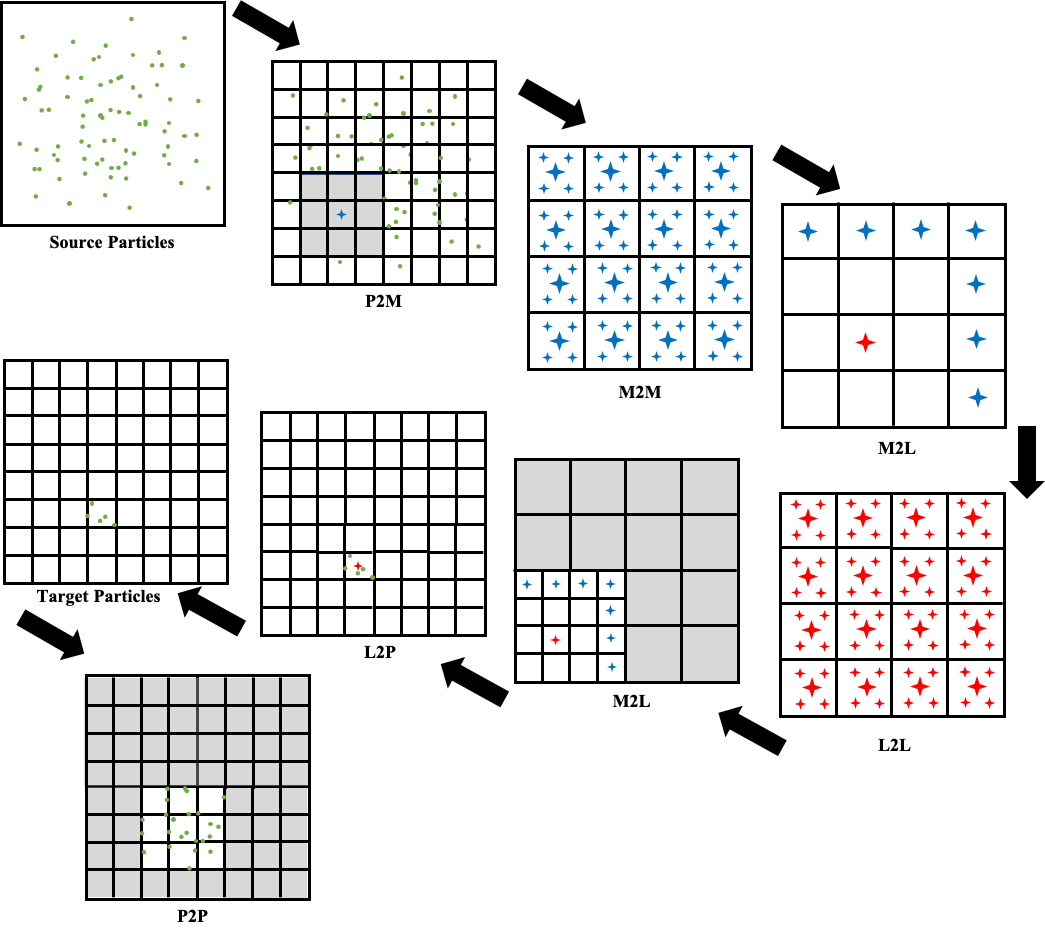
\includegraphics[width=1.1\textwidth]{introduction/main_loop.png}}
  \caption{
      The main FMM loop in two dimensions, encapsulating the upward and downward
      pass. The same set of particles are used for the sources and targets, and
      are shown in green. Local expansions are illustrated with red stars, and
      multipole expansions are illustrated with blue stars. For the P2M step the
      grey region indicates the \gls{near-field}, where this multipole expansion
      does not converge. For the M2L and P2P steps the grey region indicates
      box interactions already compressed and available via the translation or
      direct usage of local expansions. The larger/smaller stars in the M2M and
      L2L steps correspond to the parent/child expansions.
  }
  \label{fig:1_1_main_loop}
\end{figure}

\subsection{Summary}

The main practical challenge in implementing software to solve the analytic FMM
is the requirement of kernel-specific code to calculate the expansion coefficients of
(\ref{eq:1_1_multipole_expansion}) and (\ref{eq:1_1_local_expansion}). For example,
multiple different implementations already exist for Poison problems alone \cite{Greengard:1996:JCP, Etheridge:2001:SIAM}.
In software engineering terms this is inconvenient for the purposes of studying
the applications of the FMM in multiple different problem settings, as it leads to the requirement
to implement problem-specific solvers for each kernel one may encounter. This
leads to a productivity overhead in either designing a single, extensible
library, which by definition will be complex to design. Or to otherwise
maintain multiple problem-specific libraries.

The algorithm thus far described referred to as the analytic FMM is more correctly
called the non-adaptive analytic FMM. The non-adaptivity refers to the assumption that
all boxes at the leaf level are refined to the same degree, however as mentioned
in the above analysis of the algorithm, the degree of refinement is chosen such
that the number of particles in a leaf box is \textit{constant}. Therefore, If
the distribution of the particles of interest is not uniform over the computational
domain, one may be needlessly refining the boxes in some regions which may even be
empty. Therefore, although the asymptotic complexity of
the FMM is $O(N)$, it is clear that practical implementations will suffer unless
care is taken to use efficient vectorised data structures for the creation of
appropriate hierarchical tree required by the algorithm.

Additionally, there is significant scope for multiple levels of
parallelism in practical implementations. For example, the computations
for the local and multipole coefficients as well as the application of M2L, L2L
and M2M operators at a given level, are candidates for an implementation of
\textbf{\gls{task-level-parallelism}}. In addition to parallelising of each operator
application as a task, there is scope for implementing
\textbf{\gls{data-level-parallelism}} to find the expansion coefficients. For example,
Yokota and Barba \cite{Hwu:2011:MKP} demonstrate how the calculation of the P2P,
and M2L operators can be transferred to \textbf{\gls{GPU}}s using \textbf{\gls{CUDA}}.
The M2L, and P2P operators represent the largest computational bottlenecks due to
the number of such interactions in the FMM algorithm, therefore are a priority for
acceleration. For example, in three dimensions each target box has potentially
up to 189 source boxes in its \gls{interaction-list} with which to compute the
M2L operation, and for any particularly deep tree there will be roughly $O(N)$
leaf boxes, for which interactions are calculated directly. This leads to both of
these operations dominating the run-time of any \gls{FMM} implementation.

In summary, the implementation of the analytical FMM is complicated by the
fact that it is problem specific - which will also apply to any parallel
optimisation code. This in itself provides the main motivation for developing
an implementation that does not rely on explicit kernel expansions. Furthermore,
the desire for developer productivity, at the expense of hyper-optimised
implementations, is realised in this thesis by making use of Python,
a \textbf{\gls{high-level-interpreted-language}}, for our software implementation.

\section{Overview of the Kernel-Independent FMM}
\subsection{Motivation}

First introduced by Ying et. al \cite{Ying:2004:JCP}, the kernel-independent FMM (\textbf{\gls{KIFMM}})
provides an algorithm that maintains the basic recursive structure and $O(N)$
asymptotic complexity of the analytic FMM, but without the requirement for the
implementation of analytic expansions of the kernel function for each kernel.
Instead the method relies only on kernel function evaluations. This allows
software implementations to be written in an easily extensible manner for different
kernels. The main difference to the analytic FMM of Section \ref{sec:1_1_fmm_overview},
lies in the the way that source and target densities are represented, and how
the M2M, L2L and M2L operators are computed.

\subsection{Algorithm Structure \& Analysis}

For the \gls{KIFMM} presented in \cite{Ying:2004:JCP} the \gls{far-field}, $\mathcal{F}^B$, and
\gls{near-field}, $\mathcal{N}^B$, have precise specifications. For a given box $B$
centered at $\mathbf{c}$ with sides of length 2$r$, $\mathcal{N}^B$ is a box
centered at $\mathbf{c}$ with sides of length 6$r$. The \gls{far-field} is then
defined as $\mathbb{R}^d / \mathcal{N}^B$, where $d$ is spatial dimension.
Here, $B$ is in the \gls{near-field}. Consider the potential in the \gls{far-field} $\mathcal{F}^B$, generated by a
set of \gls{source-particles}, described by \textbf{\gls{source-densities}}
$\{\phi_i, \> i \in I^B_s \}$ where $I^B_s$ is the set of indices for the \gls{source-particles}
in box $B$\footnote{This notation matches that used in \cite{Ying:2004:JCP}
in order for ease of reference.}. Specifying the indices for the \gls{source-particles}
specifically to make it clear that they may be distinct from the \gls{target-particles}.
These \gls{source-particles} can be equivalently described with an \textbf{upward \gls{equivalent-density}}
distribution $\phi^{B,u}$ supported at discrete points on an \textbf{upward \gls{equivalent-surface}}
$\mathbf{y}^{B, u}$ that encloses the set of source particles. The KIFMM relies
on the assumption that the potential produced by the equivalent densities is smooth,
which is guaranteed in the case that $\mathbf{y}^{B,u}$ does not overlap with the
far-field $\mathcal{F}^B$ \cite{Ying:2004:JCP}, furthermore the requirement that
$\mathbf{y}^{B,u}$ must enclose all particles in $B$ leads to the requirement
that it must also not overlap with $B$. For second-order linear elliptic
\textbf{\gls{PDE}}s, for which the KIFMM is defined,
and of which equation (\ref{eq:poisson}) is an example, the solution for the
potential in the far field, which can be seen as an exterior Dirichlet problem,
is guaranteed to be unique \cite{Ying:2004:JCP}. Therefore, the potentials
induced by the source particles and the equivalent densities satisfy are
guaranteed to be equivalent in the far field $\mathcal{F}^B$ if they coincide
at the boundary of the far field $\mathcal{F}^B$, or anywhere between the boundary
of the far field and the upward \gls{equivalent-surface}. This boundary is referred to
as the \textbf{upward \gls{check-surface}}, $\mathbf{x}^{B, u}$, and the entire
scheme is illustrated in figure (\ref{fig:1_2_upward_downward_surfaces}A).
The equality of the potentials from the source points and the equivalent density
can be stated mathematically as follows,

\begin{equation}
\int_{\mathbf{y}^{B,u}} K(\mathbf{x}, \mathbf{y})\phi^{B, u} d\mathbf{y} = \sum_{i \in I_s^B} K(\mathbf{x}, \mathbf{y})\phi_i = q^{B, u} \> \> \text{for any} \> \> \mathbf{x} \in \mathbf{x}^{B, u}
\label{eq:1_2_p2m}
\end{equation}

\begin{figure}[!h]
    \centering
    {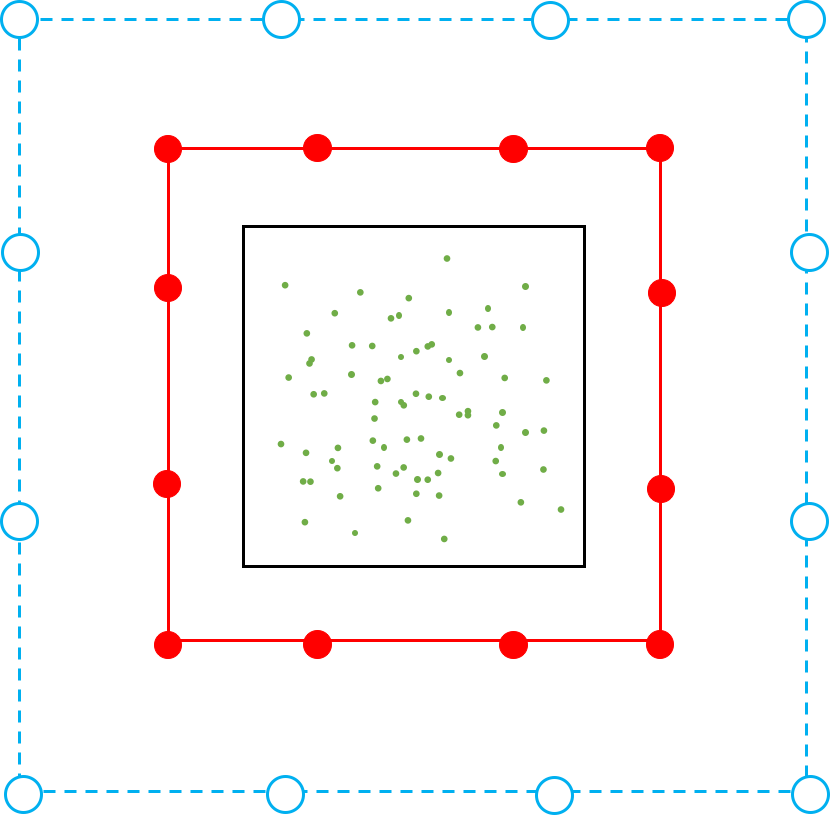
\includegraphics[width=0.3\textwidth]{introduction/upward_surface.png}}
    \hfill
  {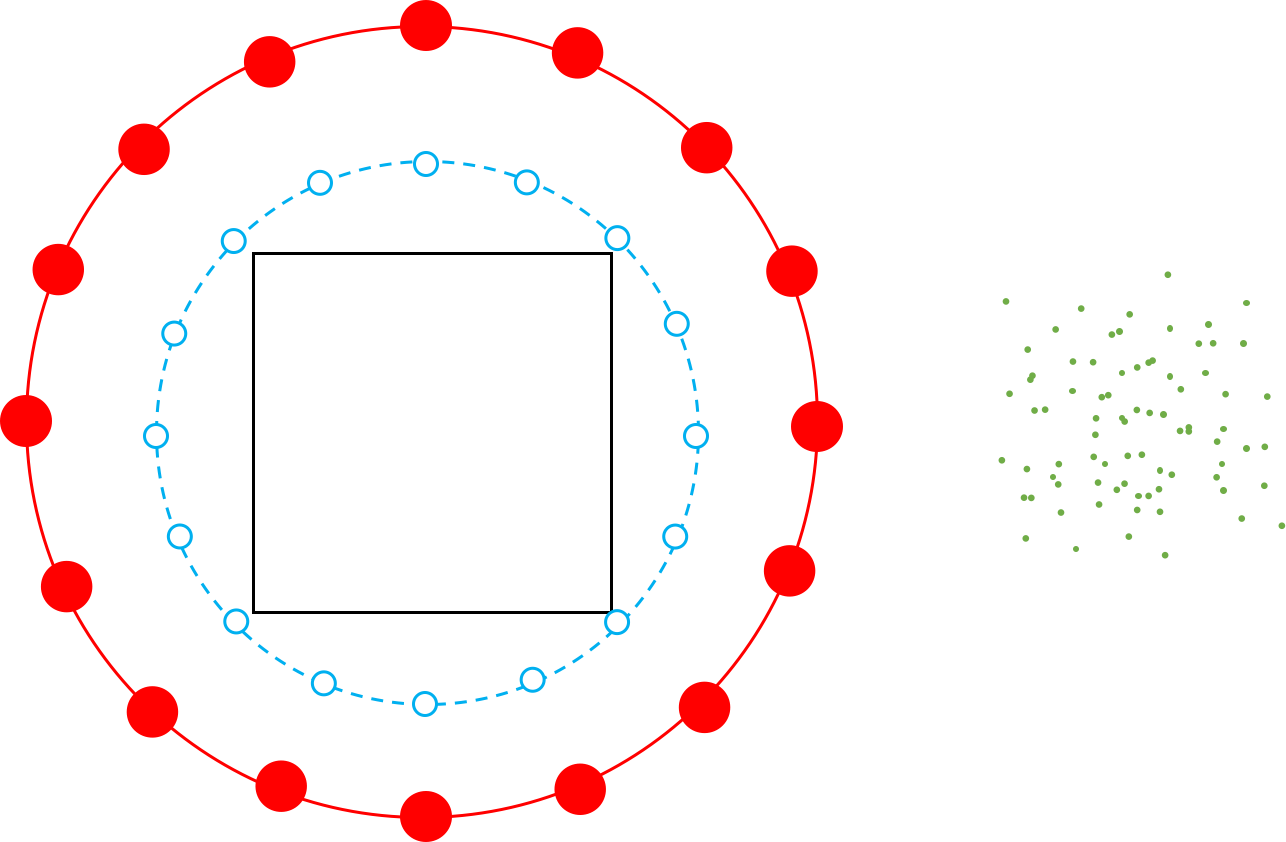
\includegraphics[width=0.4\textwidth]{introduction/downward_surface.png}}
  \vspace{0pt}
  \caption{Cross section of three dimensional cubic upward/downward equivalent and
    check surfaces. Source points are denoted by green circles. Red solid lines
    denote equivalent surfaces, and blue checked lines denote check surfaces.
    The black solid line defines the box $B$. This figure is adapted directly from \cite{Ying:2004:JCP}.}
  \label{fig:1_2_upward_downward_surfaces}
\end{figure}

where the integral form of (\ref{eq:n_body_problem}) is used for the summation of
the contribution from the equivalent densities, and $q^{B, u}$ is referred to as
the \textbf{upward \gls{check-potential}}, with the other symbols taking their previous
definitions. One can define a very similar scheme for the case in which the source
densities are in $\mathcal{F}^B$, as a potential induced by a
\textbf{downward \gls{equivalent-density}} $\phi^{B,d}$ supported at discrete points
on a \textbf{downward \gls{equivalent-surface}} $\mathbf{y}^{B,d}$. This surface
needs to be located between the boundary of $\mathcal{F}^B$ and $B$, and again
as the solution for interior Dirichlet style problems for the types of PDEs
considered in this thesis is also unique \cite{Ying:2004:JCP}, one can equate the potentials generated
by the source points with that generated by the equivalent densities at some surface
between $\mathbf{y}^{B,d}$ and $B$. This surface is called the \textbf{downward \gls{check-surface}},
$\mathbf{x}^{B,d}$, and a corresponding mathematical statement of the equality of
the potentials can be written as follows,

\begin{equation}
    \int_{\mathbf{y}^{B,d}} K(\mathbf{x}, \mathbf{y})\phi^{B, d} d\mathbf{y} = \sum_{i \in I_s^{\mathcal{F}^B}} K(\mathbf{x}, \mathbf{y})\phi_i = q^{B, d} \> \> \text{for any} \> \> \mathbf{x} \in \mathbf{x}^{B, d}
    \label{eq:1_2_p2l}
\end{equation}

where $I_s^{\mathcal{F}^B}$ represents the indices of source points in the \gls{far-field}
of $B$, and $q^{B, d}$ is the \textbf{downward \gls{check-potential}}.

The equation (\ref{eq:1_2_p2m}) is an Fredholm integral
equation, of the first kind, and it's clear that its solution $\phi^{B, u}$
can be seen to be equivalent to the multipole expansion for the \gls{source-particles} contained in $B$. Therefore,
(\ref{eq:1_2_p2m}) can be seen to be correspond to the \gls{P2M}
operation. Similarly, the solution of (\ref{eq:1_2_p2l}) can be seen
to correspond to a particle-to-local, or P2L operation. Crucially, this method of solving
a set of linear equations to find equivalents of the multipole and local expansions
does not depend on finding a series expansion of a kernel function, and just on its evaluation.

Using this language of equivalent densities and check surfaces, one is also able to
write operations equivalent to the M2M, L2L and M2L operations. For a box $A$
and it's parent box $B$, the M2M operation can be written as,

\begin{equation}
    \int_{\mathbf{y}^{A,u}} K(\mathbf{x}, \mathbf{y})\phi^{A, u} d\mathbf{y} =   \int_{\mathbf{y}^{B,u}} K(\mathbf{x}, \mathbf{y})\phi^{B, u} d\mathbf{y}, \> \> \text{for any} \> \> \mathbf{x} \in \mathbf{x}^{B, u}
    \label{eq:1_2_m2m}
\end{equation}

Once $\phi^{A, u}$ has been calculated for boxes at the leaf level of the tree,
one can apply (\ref{eq:1_2_m2m}) to evaluate the multipole expansions for all
the boxes containing \gls{source-particles} in the tree in a manner equivalent
to the upward pass of Section \ref{sec:1_1_fmm_overview}. The M2M operation is
illustrated in figure (\ref{fig:1_2_m2m_l2l}A).

For the downward pass, the M2L operation, between a box $B$ and a box $A$ in its
interaction list can be written as,

\begin{equation}
    \int_{\mathbf{y}^{A,u}} K(\mathbf{x}, \mathbf{y})\phi^{A, u} d\mathbf{y} =   \int_{\mathbf{y}^{B,d}} K(\mathbf{x}, \mathbf{y})\phi^{B, d} d\mathbf{y}, \> \> \text{for any} \> \> \mathbf{x} \in \mathbf{x}^{B, d}
\label{eq:1_2_m2l}
\end{equation}

This is illustrated in figure (\ref{fig:1_2_m2l}). Once the local expansions
have  been computed starting at level 2 of the tree, one can perform the L2L
operation to transfer the local expansion of a parent box to its children,
for a box $A$ and it's child $B$, which can be written as,

\begin{equation}
    \int_{\mathbf{y}^{A,d}} K(\mathbf{x}, \mathbf{y})\phi^{A, d} d\mathbf{y} =   \int_{\mathbf{y}^{B,d}} K(\mathbf{x}, \mathbf{y})\phi^{B, d} d\mathbf{y}, \> \> \text{for any} \> \> \mathbf{x} \in \mathbf{x}^{B, d}
    \label{eq:1_2_l2l}
\end{equation}

\begin{figure}[!h]
    \centering
    {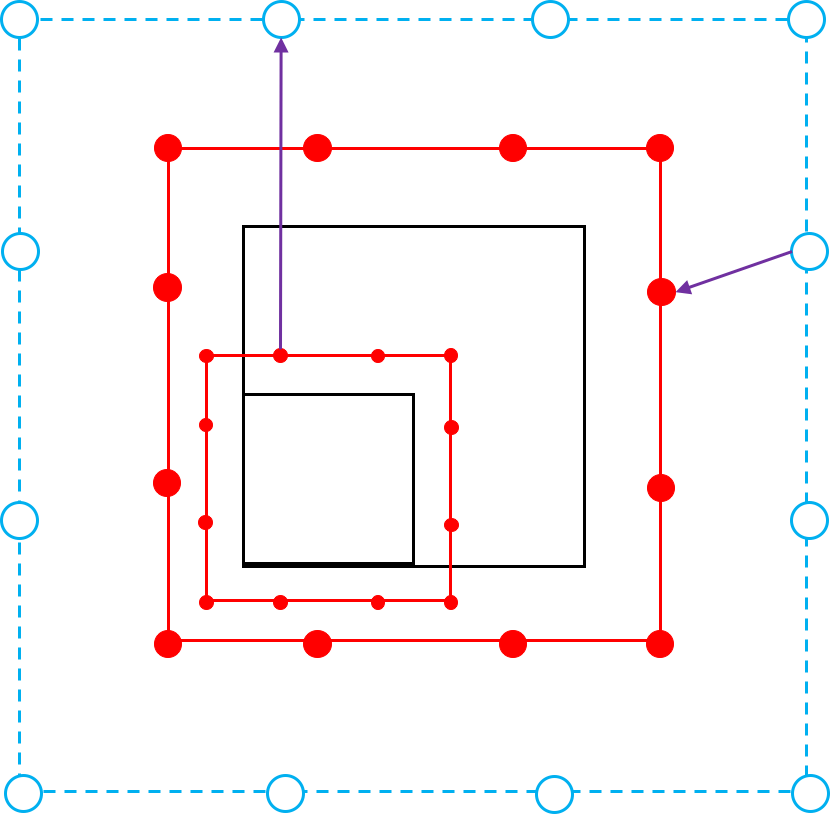
\includegraphics[width=0.4\textwidth]{introduction/kifmm_m2m.png}}
    \hfill
  {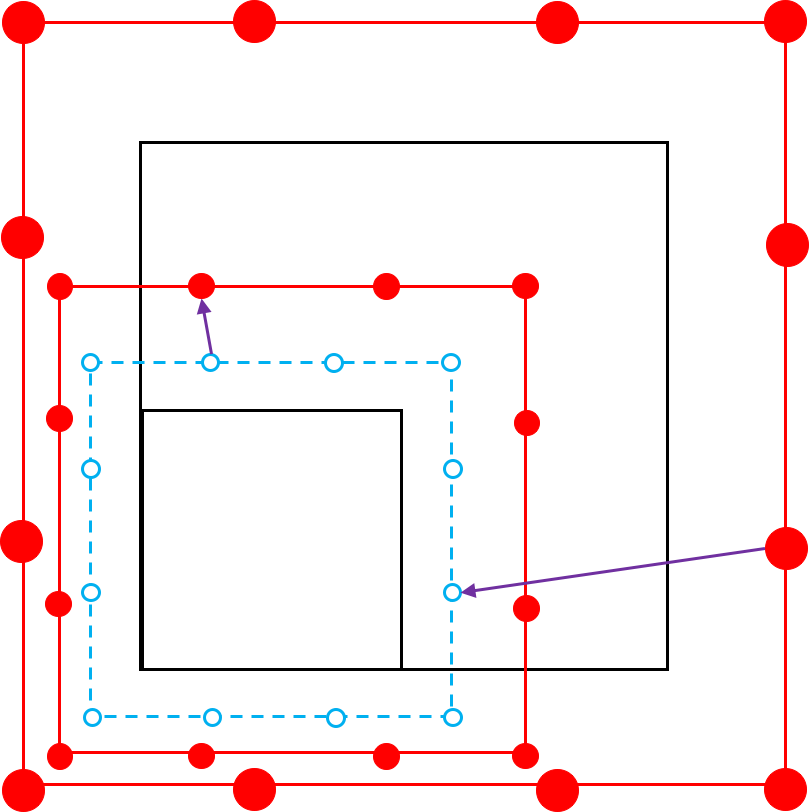
\includegraphics[width=0.4\textwidth]{introduction/kifmm_l2l.png}}
  \vspace{0pt}
  \caption{Cross section of three dimensional cubic surfaces. The (A) M2M operation and (B) L2L operation. Red solid lines
  denote equivalent surfaces, and blue checked lines denote check surfaces.
  The black solid line defines the box $B$. This figure is adapted directly from \cite{Ying:2004:JCP}.}
  \label{fig:1_2_m2m_l2l}
\end{figure}

The M2M, L2L and M2L operations are illustrated using cubic surfaces in figure (\ref{fig:1_2_m2m_l2l})
The reason for using cubic check and equivalent surfaces are for ease of integration
in the case where the discretisation points chosen are from a regular Cartesian
grid.

\begin{figure}[!h]
    \centering
    {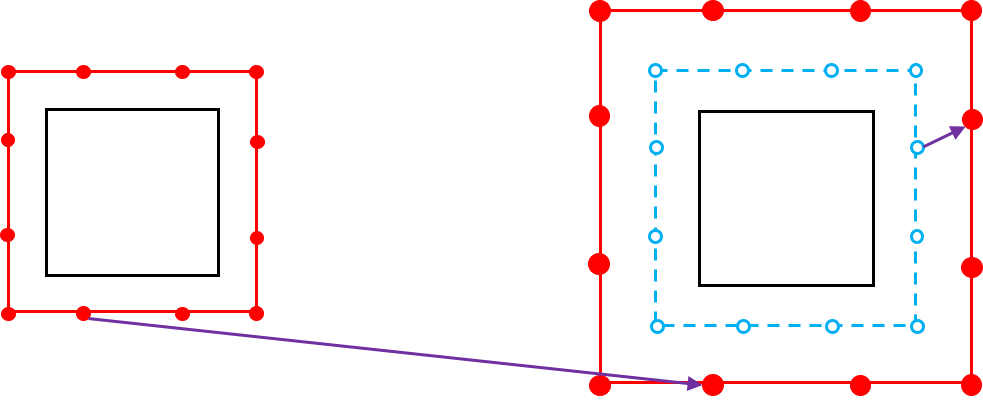
\includegraphics[width=\textwidth]{introduction/kifmm_m2l.png}}
    \caption{Cross section of three dimensional cubic surfaces for the M2L operation.
    Red solid lines denote equivalent surfaces, and blue checked lines denote check surfaces.
    The black solid line defines the box $B$.}
  \label{fig:1_2_m2l}
\end{figure}

In principle, it is now possible to replace the kernel function expansions with
the appropriate solutions of the integral equations (\ref{eq:1_2_p2m}),
(\ref{eq:1_2_m2m}), (\ref{eq:1_2_m2l}) and (\ref{eq:1_2_l2l}). However all of
the above equations are ill-conditioned, as they are ill-posed and in general infinite
dimensional problems, and therefore require appropriate regularisation in order to solve.
Consider the following general statement of the first-kind Fredholm equation
that each of the above operations requires,

\begin{equation}
K \phi = q
\label{eq:1_2_first_kind_fredholm}
\end{equation}

This expression reflects the fact that in practical implementations these continuous
integrals are discretised as matrix-vector products. Here $K$ refers to a
`kernel matrix', which can be found via numerical quadrature, $\phi$ is a vector
of equivalent density to be found, and $q$ is a known vector containing the check
potential. The reason for using cubic surfaces is the availability of simple
quadrature rules to integrate over the faces of each surface. The specifics of
the surfaces used in PyExaFMM is discussed in greater detail in Chapter 2,
Section \ref{sec:2_3_operator_caching}. One can use Tikhonov regularisation to
write the solution,

\begin{equation}
\phi = (\alpha I + K^*K)^{-1}q
\label{eq:1_2_tikhonov}
\end{equation}

where $\alpha$ is an appropriate regularisation parameter, and $I$ is the identity
matrix. This equation, a second-kind Fredholm equation, can be solved in numerous
ways. The authors of \cite{Ying:2004:JCP} make use of a Nystroem method, and indicate
the possibility of using either Galerkin or Collocation methods. For ease of
implementation, a simpler approach is to instead approximate the solution using a pseudoinverse
estimated from a Singular Value Decomposition, or \textbf{\gls{SVD}}. This
approach is adapted from the current C++ implementation of the \gls{KIFMM}, ExaFMM-t,
from the ExaFMM project \cite{exafmm}.

Consider the SVD of a matrix $A$, with $m$ rows and $n$ columns,

\begin{equation}
    A = U \Sigma V^*
\end{equation}

where as usual $U$ is the left singular matrix, $V$ is the right singular matrix
and $\Sigma$ is a diagonal matrix whose elements are the singular values of $A$.
We can write an approximate pseudoinverse of $A$ as \cite{Trefethen:1997:SIAM},

\begin{equation}
    A^\dagger = V \Sigma^\dagger U^*
\end{equation}

here, $A^\dagger$ has $n$ rows and $m$ columns, and $\Sigma^\dagger$ is formed
by taking the reciprocal of all the diagonal elements. Furthermore, to ensure
numerical stability for this reciprocal calculation, one can choose to filter
out components of $V$ and $U^*$ if their singular values smaller than a specified
tolerance. The justification of the choices for the regularisation parameter
$\alpha$ and the tolerance for the pseudoinverse are discussed in detail in
Chapter 2, Section \ref{sec:2_3_operator_caching}. In terms of the asymptotic complexity of the \gls{SVD},
as the singular values/vectors are iterated through once in a straightforward
manner to find the pseudoinverse, the complexity of this operation is at most $O(N)$,
where $N$ is the number of singlar values of $A$.

The \gls{KIFMM} algorithm shares almost all of its algorithmic steps with the analytic \gls{FMM}, the
main novelties are the least-squares solves (\ref{eq:1_2_tikhonov}) to compute
the required expansions of each box at each step of the algorithm. In turn
these solves require the computation of the check and equivalent surfaces involved,
as well as the numerical quadrature over the equivalent/source densities to compute
the required check potentials. However, the the matrix to be inverted
in the M2M operation as well as the L2L operation are very similar, which can
be seen from figure (\ref{fig:1_2_m2m_l2l}). In fact, if
the upward \gls{check-surface} is chosen to coincide with the downward
\gls{equivalent-surface}, and the upward \gls{equivalent-surface} is chosen to
coincide with the downward \gls{check-surface}, the matrix to be inverted for the M2M
operation is the transpose of the matrix to be inverted for the L2L operation,
except for a scaling factor dependent on the level of the Octree the surfaces
are created in. This scaling factor is easy to identify, and for the model problem of
three dimensional electrostatics with a Laplace kernel, the scaling factor between
kernel matrices evaluated at two adjacent Octree levels, $l$, is $K^{l+1} = 2K^l$.
Similarly, the required matrix inverse for the L2L and M2L operations exactly coincide
except for a scaling factor. Therefore, practical implementations
need to compute at most one matrix inversion which can be cached. This can then
be scaled and applied as required at each step of the algorithm. Furthermore,
for the Laplace kernel specifically, the scaling factors are present on both sides
of the equations (\ref{eq:1_2_m2m}) and (\ref{eq:1_2_l2l}), cancelling each other out.
This means that the M2M and L2L operations can also be calculated between just one
parent box and its respective child boxes, and cached for later use.

Considering the asymptotic complexity of the inverse, its calculation is bound
by a term proportional to the number of singular values of the kernel
matrix, which in turn is dependent on the number of quadrature points chosen for
the check and equivalent surfaces. Therefore as long as this number of quadrature
points is kept small, the pseudoinverse does not effect the asymptotic complexity
of the \gls{KIFMM}. The remainder of the M2M, M2L and L2L operations are bound by
the complexity of computing a matrix vector product between the calculated inverse
matrix and the check potentials, which is resultantly also not impactful on the
algorithm's asymptotic complexity as long as the requirement on the number of
quadrature points is satisfied. As the other algorithmic analysis from
Section \ref{sec:1_1_fmm_overview} remains the same, we can see approximately how
the $O(N)$ complexity is maintained for the \gls{KIFMM}.

\subsection{Summary}

The different approach of the \gls{KIFMM} leads to some different implementation
challenges in comparison to the \gls{FMM}. The key difficulty arises from the
instability in computing the matrix inverse of the kernel matrix between the
check and equivalent matrices. As mentioned, choices for the
regularisation parameter $\alpha$ as well as the tolerance for singular values
taken in the pseudoinverse are discussed with this in mind in Chapter 2, Section
\ref{sec:2_3_operator_caching}.

The ability to cache the M2M and L2L operators, after calculation for a single
parent box and its respective child boxes, leaves the main bottleneck to
pre-computing all the required operators as the matrix-vector products required
to compute the M2L operators. The original authors of the \gls{KIFMM}
accelerate the calculation of the M2L operation using a Fast Fourier Transform,
or \textbf{\gls{FFT}} \cite{Ying:2004:JCP}. To see why this can be done, consider
the surfaces describing the M2L operation illustrated in figure (\ref{fig:1_2_m2l}),
if the downward \gls{check-surface} of the target box, and the upward
\gls{equivalent-surface} are chosen to be equivalent and lie on a regular Cartesian
grid, then the component of the M2L operation that evaluates the action of a
kernel function between these two surfaces can be considered as a convolution
between the kernel function and the equivalent density. Mathematically, if the
kernel function $K(x, y)$ depends only the difference between $x$ and $y$ as it
does for these choices of surfaces for the M2L operation, the left hand side of
(\ref{eq:1_2_m2l}) goes to,

\begin{equation}
    \int_{\mathbf{y}^{A,u}} K(\mathbf{x} - \mathbf{y})\phi^{A, u} d\mathbf{y} = q^{B, d}\> \> \text{for any} \> \> \mathbf{x} \in \mathbf{x}^{B, d}
\end{equation}

Padding the empty nodes with zeros allows us to apply the Fourier convolution theorem,
and solve for equivalent density as,

\begin{flalign}
    \phi^{A, u}(\mathbf{y}) = \mathcal{F}^{-1} \left [ \frac{\mathcal{F}(q^{B, d}(\mathbf{x}))}{\mathcal{F}(K(\mathbf{x}))} \right]
\end{flalign}

The currently available major \gls{KIFMM} implementations use this to accelerate the calculation of the
M2L operator including ExaFMM-T and PVFMM \cite{Malhotra:2015:CCP, exafmm}.  Though
reasoned in more detail in Chapter 2, Section \ref{sec:2_3_operator_caching}, we state for
the present that the expansion order $p$ is by definition proportional to the
number of quadrature points used to discretise the surface of the check and
equivalent surfaces. Specifically, PyeExaFMM follows the example of ExaFMM-T and
PVFMM, taking the relationship between $p$ and number of quadrature points, $n_q$,
to be,

\begin{equation}
    n_q = 6(p-1)^2 + 2
\end{equation}

Meaning that each surface has $O(p^2)$ points, and therefore the M2L operation
(\ref{eq:1_2_m2l}) is of $O(p^4)$ between a given target box and source box.
This FFT based method to find equivalent densities, accelerates the M2L calculation between a given target box
and a given source box to $O(p^3 \log(p))$. In PyExaFMM we use an alternative
acceleration scheme, based on low rank SVD approximations, discussed further in
Chapter 2, Section \ref{sec:2_4_svd_compression}. Therefore we defer to the
literature for further details on FFT based acceleration methods \cite{Malhotra:2015:CCP}.

The \gls{KIFMM} presents many of the same opportunities for parallel implementation
as the \gls{FMM}. In terms of \gls{task-level-parallelism}, PyExaFMM implements
parallel processing, via Python's native multiprocessing tools, for the calculation
of the M2L operations. As these calculations involve dense matrix-vector products,
they are also ideal candidates to be transferred
to a \gls{GPU} for rapid parallel evaluation in the future. PVFMM implements
\gls{task-level-parallelism} for the calculation of the M2M, L2L, and M2L
operators with \textbf{\gls{MPI}} as well as an interface with \gls{CUDA} for
processing the dense matrix-vector products. ExaFMM-T makes use of
\textbf{\gls{OpenMP}} for a similar purpose.

In summary, the key benefits of the \gls{KIFMM} lie in the ability to write
an implementation that is compatible with a wide class of kernel functions,
without evaluating the expansion coefficients. This greatly reduces the complexity
of the software design to support multiple applications of the FMM across
different problem settings. Furthermore, the formulation of the key FMM operations
as dense matrix-vector products makes it easy to map portions of the \gls{KIFMM}
to dedicated parallel hardware such as \gls{GPU}s. The fact that KIFMM logic
is not dependent on the form of the kernel function expansion, and just on kernel
function evaluations,  makes it trivial to separate the concerns of a software
implementation, and write optimisation libraries for the KIFMM independently of
the main loop (fig. \ref{fig:1_1_main_loop}) itself. The impact on software design
and architecture is signficant, and is explored further in Chapter 2 Section
\ref{sec:2_5_software_design}. This design is the key benefit of PyExaFMM
in comparison to existing \gls{KIFMM} implementations, as PyExaFMM is already
sacrificing a degree of performance via the choice of implementation language,
we are able to implement some effective software engineering principles
to ease the burden on a user in terms of debugging and expanding upon PyExaFMM.



    \chapter{Strategy for Practical Implementation}\label{chpt:2_strategy_for_practical_implementation}

\section{Bottleneck Overview}\label{sec:2_1_bottleneck_analysis}
Some of the key bottlenecks in implementing the \gls{FMM} and \gls{KIFMM}, and potential
optimisation strategies in the computation of these algorithms, have already been
discussed. This chapter adds detail to the approaches used by \gls{PyExaFMM} to tackle
the issues raised. Namely, the approach to multiprocessing and caching the \gls{M2M},
\gls{L2L} and \gls{M2L} operators is discussed in Section \ref{sec:2_3_operator_caching}, and
the acceleration of the \gls{M2L} calculation via a low-rank approximation using the \gls{SVD}
is discussed in Section \ref{sec:2_4_svd_compression}. The other significant bottlenecks
and implementation issues addressed in thus far by \gls{PyExaFMM} are the
efficient construction of tree data structure (Section \ref{sec:2_2_efficient_trees}),
and the software design considerations (Section \ref{sec:2_5_software_design}).

The twin goals in designing \gls{PyExaFMM} were ensuring the extensibility and
testability of the software. Building easily extensible and testable numerical
codes is inherently challenging, the complexity of the algorithms and continuous
nature of their results making it hard to separate the logic from application
specific implementations. As \gls{PyExaFMM} is implemented in Python, an
\textbf{\gls{interpreted}} and inherently \textbf{\gls{object-oriented-language}}, we are able to use some common and powerful
object oriented design principles to ensure extensibility. Concerns about the
overhead of using the object oriented design principles, in comparison to directly manipulating
primitives, such as those available in lower level compiled languages such as C
or C++, are misplaced for two reasons. Firstly, the implementation of Python objects
is syntactic sugar, methods and data for a given object are written into
a simple dictionary structure at run time, with the `class' syntax common to other
object oriented languages such as C++ or Java, offered for as they are familiar to
the programmer coming from such languages. Resultantly, all `primitives' such as
integers and strings in Python are actually objects by design, being quite different
in their construction from C or C++ where the programmer is given the power to
allocate memory for true primitives themselves. In Python the overhead therefore
comes from the interpreter, which transforms the source code into byte code which
is then compiled. This additional interpreter layer is the source of Pythonic overhead,
rather than the object abstraction in itself. Therefore, once the decision has
been made to use Python, there isn't a significant overhead from using object
oriented design principles, with the added benefit of increasing programmer
productivity, and easier testability. Secondly, the vast Python ecosystem of
optimised libraries for numerical computation allow for the manipulation and
allocation of primitives in memory in a manner closer to a compiled language.
Specifically, \gls{PyExaFMM} implements all of its containers with NumPy, which
offers an interface for the allocation and access of numerical data with C-like
efficiency, due to the underlying subroutines being written in C. Additionally,
\gls{PyExaFMM} uses just-in-time (\textbf{\gls{JIT}}) via the Numba library on
numeric subroutines implemented with NumPy containers. Just-in-time compilation
refers to a system which analyses the byte-code of generated by an interpreter
for repetitive operations which would benefit from compilation and caching, therefore
combining the speed benefits of compiled languages, with the flexibility of interpreted
languages. Software design choices in light of the above analysis is considered
in detail in Section \ref{sec:2_5_software_design}, and the result of code
optimisation is benchmarked in Chapter \ref{chpt:3}, section \ref{sec:3_1_benchmarking}.

As with all optimised numeric codes, \gls{PyExaFMM} relies on an efficient
vectorised datas structures, specifically an efficient representation of the tree
data structure used in the main \gls{FMM} loop. This is done via an Morton encoding,
which has the effect of translating multidimensional data to one dimension whilst
preserving the data's locality. This allows for an efficient vector representation
of box center's in a tree, and for the application of optimised numeric libraries.
The software implementation is discussed in detail in Section \ref{sec:2_2_efficient_trees}.
}

\section{Efficient Tree Implementations}\label{sec:2_2_efficient_trees}
Spatial decompositions of a set of $d$ dimensional coordinates into a single
dimension is widely applied across computational science.
From forming the basis of implementations of finite-element methods, to algorithms
for mesh refinement, and importantly in our case, $N$-body simulations
\cite{Sundar:2008:SIAM}. Spatial decompositions utilise space-filling curves,
these infinite-curves are fractal, and by increasing their `order' can be made
to `fill', or describe, a $d$ dimensional space uniquely simply by their position
along the length of the curve \cite{Campbell:2003:Williams}. This concept is
illustrated in figure (\ref{fig:2_2_multi_order}) for the Morton encoding, or a
`Z-order' encoding.  This figure illustrates the fractal nature of a Morton
encoded line, with two `orders' of line encoding plotted over one another. We see
how by using a higher order encoding, we are able to to describe each position
in the domain of the box with a greater degree of precision, by using just
the length along the encoded line as a coordinate. This variant of space-filling
curves is used by \gls{PyExaFMM} as it better preserves the proximality of data
in the encoded coordinates than most other encodings, meaning that distance
between data points in physical space is preserved to an extent by the encoding. In $N$-Body
problems that use tree data structures, the encoded line is chosen to pass through
the centre of each box in the tree, at each level. Usefullly, Morton encodings
do not have the requirement to be continuous as illustrated by figure
(\ref{fig:2_2_multi_order}), making them relatively simple to implement.

As the line is chosen to pass through the center of each quadrant of the quadtree,
 the position along the line in each quadrant of a given box can be efficiently represented
 as a pair of `binary coordinates' corresponding to the index of the quadrant the line
 passes through, as the dimensions of the box at each level are pre-defined for a
 given octree. For example, the bottom-left quadrant at the coarser level in figure (\ref{fig:2_2_multi_order})
 will have a binary coordinate of,

 \begin{equation}
     \underbrace{0}_{x}\underbrace{0}_{y},
 \end{equation}

 where $x$ and $y$ correspond to the index of the quadrant along the $x$ and $y$
 directions at this level. This encoding can be made unique for each
 quadrant in each level by adding a displacement corresponding to the number of boxes so far
 encoded at all coarser levels. For example, the first encoded box, which in figure (\ref{fig:2_2_multi_order})
 corresponds to the binary coordinate $00$ will have a displacement of 0.
 This leaves this first box with a Morton encoded position, or \textbf{\gls{key}}
 of 0 in base ten. Similarly, the encoding for the bottom-left box at the finer
 level in figure (\ref{fig:2_2_multi_order}) will have binary coordinates of,

 \begin{equation}
    \underbrace{00}_{x}\underbrace{00}_{y},
\end{equation}

Four bits are needed, two each for the $x$ and $y$ coordinate, as there are 16
 quadrants at this level. The displacement due to the number of boxes encoded at
 previous levels of 4 \footnote{As is common in computer science, we begin indexing at 0, rather than 1.},
therefore it's Morton \gls{key} in base ten will be $4$. This concept is easily
extended to three dimensions, and is illustrated in
figure (\ref{fig:2_2_morton_encoding}) at level 1 of an octree. Here the binary
coordinates simply contain three bits, for the $xyz$ octant of a given cube
in the octree, and the displacement mechanism is entirely analogous with the
two dimensional case.

The binary coordinates of Morton encoded octants make it easy to perform simple
bitwise shift and comparison operations, to assign source and \gls{target-particles} to the Morton key
that encodes the octant they lie in for each level of a given octree, as well as traverse the levels of
the octree. Specifically, \gls{PyExaFMM} makes use of a \textit{linear} Morton encoding, meaning that it assigns
all particles to the keys of boxes they occupy at a maximum depth which has been refined to a
pre-defined leaf level of the desired octree. It does so by assuming that the
leaf level of the octree describing the domain of interest is partitioned into equal
sized leaf boxes, and checking the relative coordinates position of each particle
with respect to the expected indices of the leaf boxes. Furthermore, this operation only provides
a set of keys at the leaf-level which are non-empty, allowing \gls{PyExaFMM} to
ignore the remainder of the space covered by the domain of the octree. Once this
linear representation has been found, and the non-empty boxes containing
source and \gls{target-particles} identified, it's easy to traverse the octree
to find which ancestor boxes particles lie in by simply subtracting the appropriate
offset due to the box's position along the entire Morton encoded line, and adding a new offset at
at level of the ancestor box. The inverse operation can be done to provide the set
of keys corresponding to the descendent boxes for a given box. In terms of the
\gls{FMM} and \gls{KIFMM} algorithms, the above operations can be extended trivially
in simple combination to pre-compute \gls{interaction-list}s for each box, containing
only source boxes which aren't empty, as well as to find \gls{near-neighbours} of
a given box at a given level of the octree.

The power of encoding the domain of the octree lie in the optimisation opportunities
that arise. \gls{PyExaFMM} works entirely in terms of encoded Morton keys, using
them to lookup the correct precomputed operators, and store computational results against.
The ability to store an Morton encoding in Numpy vectors makes it possible to use
Numba's \textbf{\gls{JIT}} functionality to precompile the bitwise
operations, which are used heavily in \gls{PyExaFMM}'s implementation of the \gls{KIFMM}
main loop, mainly to traverse the octree. Properties of \gls{JIT} compilation are
elaborated on in Section \ref{sec:2_5_software_design}, and the speedup offered
by just-in-time compilation is benchmarked in Chapter \ref{chpt:3}, Section
\ref{sec:3_1_benchmarking}. Most significantly, this implementation detail
represents the first step towards optimising tree construction, with the
field of optimising highly-parallel tree constructions for octrees potentially containing
$10^9$ or more octree boxes, being an active area of research \cite{Sundar:2008:SIAM,Malhotra:2015:CCP}.
For example, the authors of PVFMM, one of the major C++ \gls{KIFMM} implementations,
evenly distribute the load of encoding particles for particularly deep octrees across
multiple processes using \gls{MPI} \cite{Malhotra:2015:CCP}. For highly non-uniform
data distributions the non-adaptive implementation of \gls{PyExaFMM} currently
will wastefully refine regions of the octree with a low density of particles, major
open source \gls{KIFMM} implementations thus implement adaptive tree refinement,
with different sized leaf boxes in different regions of the domain decsribed by
the octree \cite{Ying:2004:JCP, Malhotra:2015:CCP, exafmm}.

\begin{figure}[!h]
    \centering
    {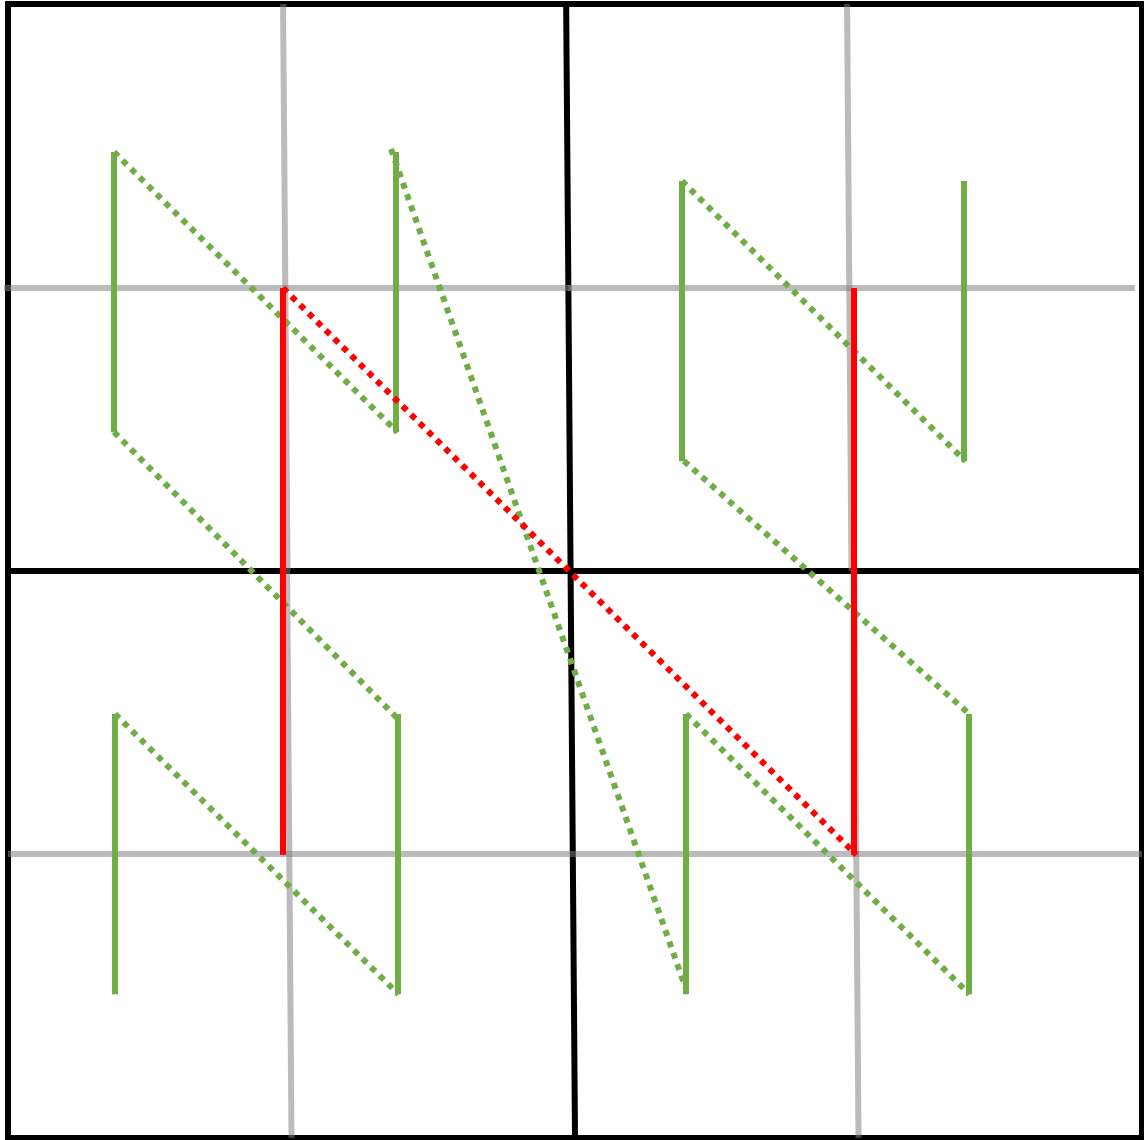
\includegraphics[width=0.45\textwidth]{chapter2/2_order.png}}
    \vspace{0pt}
    \caption{
        Two orders of Morton encoded lines in two dimensions for a quadtree across
        two adjacent levels. The red line encodes the center of the quadrants at the higher level,
        and and the green line encodes the corresponding points a level deeper.
        The dashed line indicates the order in which displacements are calculated
        in the encoding where the line is discontinuous.
    }
    \label{fig:2_2_multi_order}
\end{figure}


\begin{figure}[!h]
    \centering
    {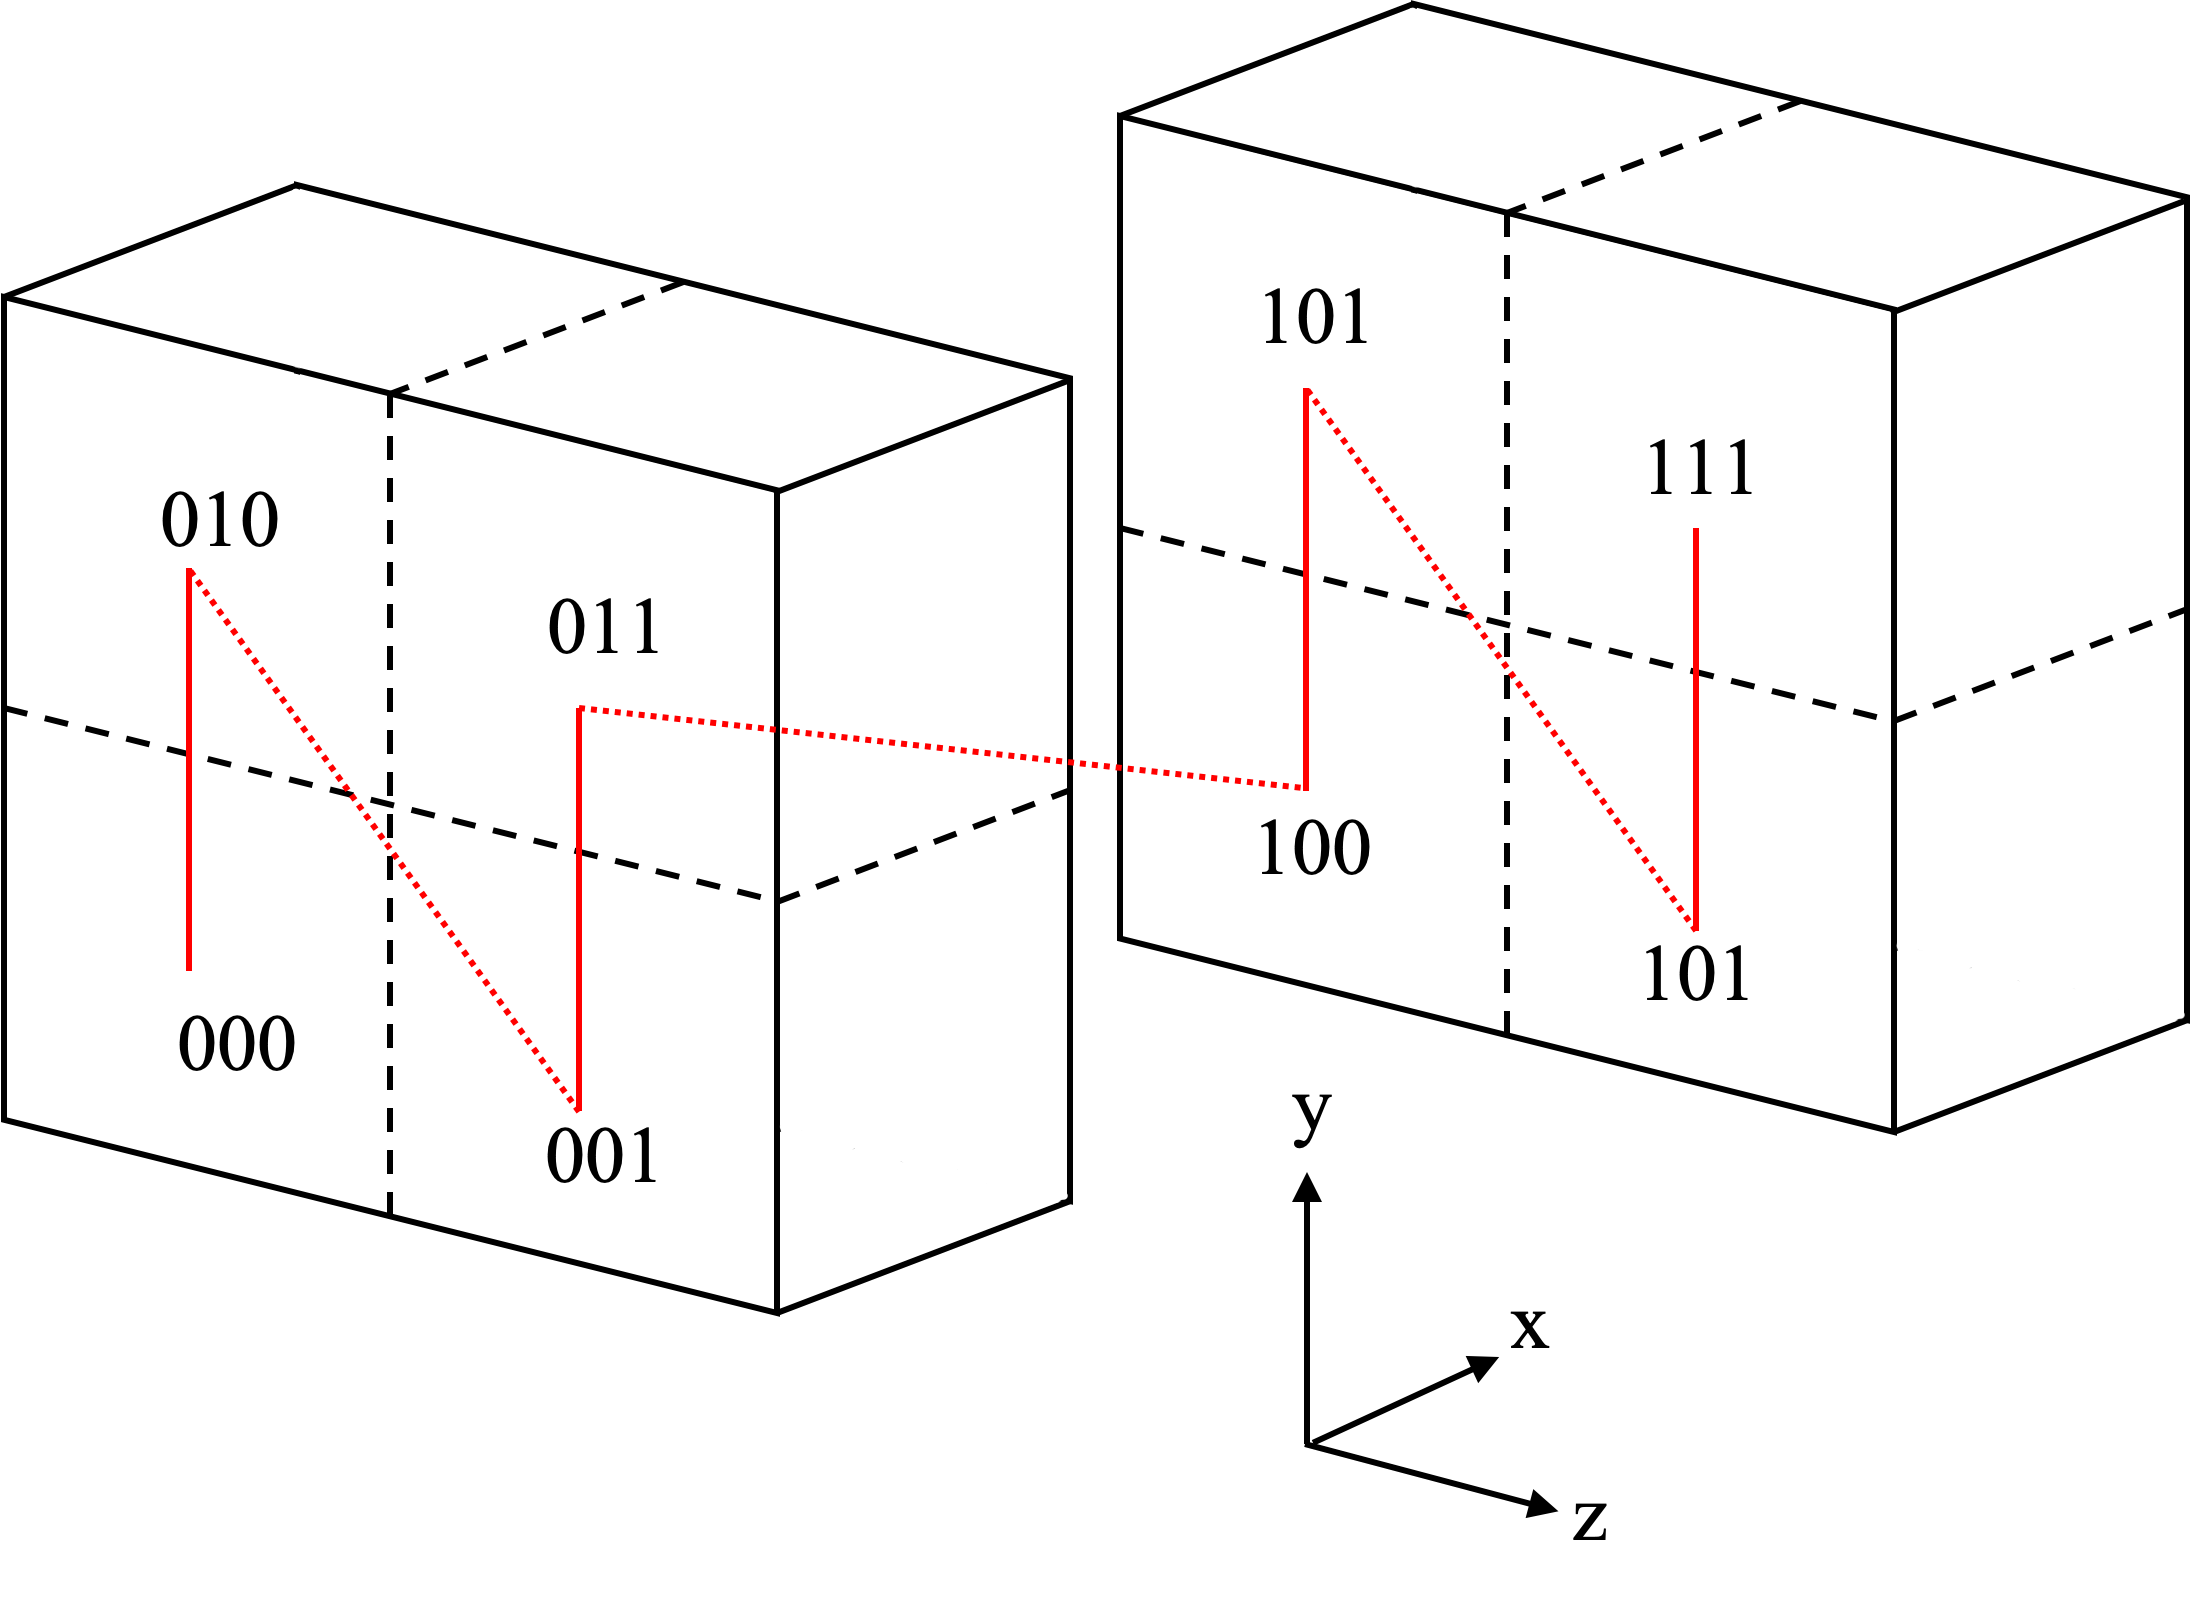
\includegraphics[width=0.65\textwidth]{chapter2/z_encoding.png}}
    \vspace{0pt}
    \caption{
        Morton encoding at level 1 of domain described by an non-adaptive octree.
        The two `layers' of the octree at this level have been broken apart
        in order to illustrate the encoded line. The Morton keys are written
        as binary coordinates in each octant.
    }
    \label{fig:2_2_morton_encoding}
\end{figure}}

\section{Operator Caching and Multiprocessing}\label{sec:2_3_operator_caching}
Practical implementations of the \gls{KIFMM} rely on the creation of efficient
surfaces used in the calculation of kernel matrices, as well as a stable method for
computing the inverse of these kernel matrices. The former problem naturally leads
to the implementation of caching code to store, re-use, and scale operator matrices
as appropriate. Whereas the latter requires the implementation of a stable method to
solve the system of linear equations for each \gls{KIFMM} operator. As mentioned
in Chapter \ref{chpt:1_introduction}, Section \ref{sec:1_2_kifmm_overview}, \gls{PyExaFMM} uses
a pseudoinverse computed via an SVD to solve this linear system. This section
provides the implementation details used to address both of these issues.

\gls{PyExaFMM} uses cubic surfaces for all check and equivalent surfaces discretised
to the same degree, this follows the precedent set by the original authors \cite{Ying:2004:JCP}, and
allows for the application of simple quadrature rules to calculate the various
operator integrals such as those in equations (\ref{eq:1_2_m2m}), (\ref{eq:1_2_m2l})
and (\ref{eq:1_2_l2l}). In fact, as the number of quadrature points is generally
chosen to be relatively low \gls{PyExaFMM} uses a direct computation to
compute the required integrals. Specifically, an order $p$ expansion results in,

\begin{equation}
    n_q =  6(p-1)^2 + 2
    \label{eq:2_2_quadrature_points}
\end{equation}

where $n_q$ is the number of quadrature points on a given surface. This equation can be
justified from the enforcement of the fact $p$ quadrature points are placed on the corners
of the cube, as well as being placed evenly along each edge of the cube. Similarly the
interior of each face of the cube is discretised to have quadrature points that form
a uniform Cartesian grid with the points at the edges and corners. Therefore,
by over-counting the nodes on the edge the 6 sides of the cube lead to $6p^2$ quadrature
points, however each corner point is over-counted three times, and the quadrature points
in the interior of a edge are over-counted twice. This leads to $6p^2 - 12(p-2) - 16$,
which is equivalent to (\ref{eq:2_2_quadrature_points}), however computed with more operations.
Therefore even for an order $p=9$ expansion, which can be employed to compute
potentials to 9 digits of accuracy with respect to a direct computation
\cite{Malhotra:2015:CCP}, there are just 386 quadrature points on a given check
or equivalent surface.

The operators associated with the \gls{KIFMM}, described by equations
(\ref{eq:1_2_m2m}), (\ref{eq:1_2_m2l}) and (\ref{eq:1_2_l2l}) are of the general
form,

\begin{equation}
    K_A\phi^A = K_B\phi^B
\end{equation}

where $K_A$ and $K_B$ are integral operators describing the action of the kernel
between two surfaces describing their given box, and can be discretised into
matrices by performing numerical quadrature but storing the element-wise results
as matrix elements; and $\phi^A$ and $\phi^B$ are equivalent densities, one of
which is generally unknown and sought. This can be reformulated as,

\begin{equation}
    \phi^A = (K_A)^{-1}K_B\phi^B
    \label{eq:2_3_general_operator}
\end{equation}

in the case $\phi^B$ is known and $\phi^A$ is sought. For the remainder of this
thesis, the quantity $(K_A)^{-1}K_B$ will be referred to as an \textbf{\gls{operator-matrix}},
for example the `M2L operator matrix', and so forth. This is a useful quantity
to cache, in comparison to just storing the inverse and the kernel matrices separately,
as we can just apply the M2L operator matrix to the known source density in order
to calculate the unknown source density in a single matrix-vector product.

As described in Chapter \ref{chpt:1_introduction}, Section \ref{sec:1_2_kifmm_overview}, one
can take advantage of the similarities between the nature of the calculation of
(\ref{eq:2_3_general_operator}) for the \gls{M2M} and \gls{L2L} operator matrices, if
the check and equivalent surfaces in both cases are chosen correctly. Specifically,
if the upward check surface is chosen to coincide with the downward equivalent
surface, and the upward equivalent surface is chosen to coincide with the
downward check surface, the matrix $K_A$ in for both cases are the transpose of
of one another, with the addition of a scaling factor to account for the fact
that $K_A$ describes the surfaces at the child level for a the \gls{L2L} operation,
versus at the parent level for the \gls{M2M} operation. Furthermore as each of these
operations is only relative between a parent box and its respective children, one
can just compute all M2L and L2L operator matrices for a given parent and its
respective children and re-use at any level of an octree. \gls{PyExaFMM} therefore
computes, and caches, the M2M and L2L operators and saves them alongside the
corresponding child Morton \gls{key} of the child box involved in their calcualtion,
 this can be looked up as needed during the \gls{KIFMM} main loop. For the M2L
 matrices, an alternative approach is taken, \gls{PyExaFMM} computes
and caches all M2L operator matrices for all source boxes in a given target box's
interaction list for all target boxes at all levels. Presently, this computation is distributed across
the available processors of multicore machine
with Python's native multiprocessing utilities. However, dense matrix-vector
product operations, such as those required to find the \gls{M2L} operator
matrices, are good candidates for offloading to \gls{GPU}s. Modern \gls{GPU}s
consist of up to $O(10^3)$ processor cores at the higher end,
in comparison to $O(10)$ on an average desktop work work station's CPU
\cite{Hwu:2011:MKP}. Roughly speaking, this number of cores allows for massive task level parallelism,
and works especially well for single-instruction multiple-data (\gls{SIMD}) type tasks, in which
a single instruction is passed to each process alongside a small amount of data on which it
is required to operate. A dense matrix vector product is therefore an ideal
candidate for GPU acceleration, due to the independence of the calculation between each row
of the matrix and the vector, each of which can be broken up again into independent element-wise
products. As there are up to 189 M2L operator matrices for a given
target box, corresponding to the potential length of a target box's interaction
list in three dimensions \cite{Ying:2004:JCP}, this problem can be reformulated
as a linear system involving the matrix vector products of M2L operator matrices
with their respective source equivalent densities,

\begin{equation}
    \left [ A_1 | A_2 | ... | A_I \right] \begin{bmatrix} \phi_1 \\ \phi_2 \\  ... \\  \phi_I \end{bmatrix} = \begin{bmatrix} q_1\\ q_2\\  ... \\  q_I \end{bmatrix}
    \label{eq:2_3_concatenated_m2l}
\end{equation}

where $\{A_i | i \in [1, 2, ..., I]\}$, are the M2L operator matrices for a given
source and target box pair and $I$ is the size of a given
target box's interaction list. Additionally, $\{\phi_i | i \in [1,2, ..., I]\}$ and $\{q_i | i \in [1,2, ..., I]\}$
are the source box's equivalent density and the corresponding check potential vectors
respectively. The concatenated operator matrix for this system can be compressed, and still
provide accurate results. This is the focus of Section \ref{sec:2_4_svd_compression},
where it's shown how \gls{PyExaFMM} uses a low-rank estimate of this matrix using
an \gls{SVD}. This compression has the potential to offer a large saving in terms
of the size of the cached M2L operator, and the time complexity of its application
on source densities. Therefore, the decision to compute the \gls{M2L} operators for
all target boxes is taken with the potential for future GPU acceleration and
compression techniques in mind.

The values chosen for the size of the for the size of the upward/downward
check and equivalent matrices are taken with reference to \cite{Malhotra:2015:CCP},
as the authors empirically find them to achieve good results. Specifically,
the radius\footnote{It's conventional in FMM literature to refer to the half-side
length of a box as the `radius'}, of the upward check surface and downward equivalent
surface of a given box is set to be 2.95 times the radius of the box, and the radius of
upward equivalent surface and downward check surface are set to be 1.05 times the radius
of the given box. This parameter choice is common to both major C++ implementations of
of the \gls{KIFMM} \cite{exafmm,Malhotra:2015:CCP}.

As mentioned, the required operator matrices are loaded from disk at run-time, ready to
be used by \gls{PyExaFMM}. Currently, objects corresponding to cached \gls{M2L}
matrices are simple serialised to be loaded in their entirety at run time by
\gls{PyExaFMM}. However, the translation of the cache to HDF5 based storage is
an area of future extension, and has been implemented
for the storage of the \gls{M2M} and \gls{L2L} operator matrices. HDF5 offers an
interface for loading slices of large datasets that may be stored on disks, allowing
for rapid read times for subsets of a data, even if the underlying dataset
is of the order of gigabytes \cite{Wasser:NSF}. Furthermore, HDF5 allows for the
hierarchical storage of numeric arrays, this amounts to creating
a database like structure on disk which can store numeric arrays of different
dimensions.

The  benchmark figures for the potential speedup offered by the above optimisations
implemented in \gls{PyExaFMM}, namely multiprocessing for the \gls{M2L} operators
and the usage of HDF5 vs object serialisation for large datasets are given
in Chapter \ref{chpt:3}, Section \ref{sec:3_1_benchmarking}.

As discussed in Chapter \ref{chpt:1_introduction}, Section \ref{sec:1_2_kifmm_overview},
the calculation of (\ref{eq:2_3_general_operator}) is ill-conditioned, therefore
\gls{PyExaFMM} uses a Tikhonov regularisation scheme in combination with an SVD
to to calculate the inverse of the operator matrices, which is adapted from the
implementation of ExaFMM-T and PVFMM \cite{Malhotra:2015:CCP, exafmm}.

Consider the SVD of a given operator matrix,

\begin{equation}
    K_A = U \Sigma V^*
\end{equation}

with a pseudoinverse of

\begin{equation}
    K_A^\dagger = V \Sigma^{-1} U^*
\end{equation}

the inversion of the diagonal matrix of singular values can be regularised as,

\begin{equation}
    \Sigma^{-1} = \underbrace{(\alpha I + \Sigma^*\Sigma)^{-1}}_{\Sigma_{\text{reg}}}
    \label{eq:2_4_regularised_general_operator}
\end{equation}

a pseudoinverse using an \gls{SVD} is then calculated for this matrix, in which
singular vectors corresponding to `small' singular values less than a specified
tolerance are filtered out of the final approximation in order to maintain
numerical stability. This tolerance value is in practice set to be a number close
to machine precision, and \gls{PyExaFMM} uses a value of $\text{tol} = 4 \cdot \text{EPS} \cdot \max (\Sigma_{\text{reg}})$,
where EPS is machine precision, and $\max (\Sigma_{\text{reg}})$ is the largest
entry in $\Sigma_{\text{reg}}$. This has been determined empirically to provide
stable results. The regularisation parameter $\alpha$ is also determined empirically,
and a value proportional to the largest singular value of $K_A$, where
$\alpha=0.075 \cdot \max(\Sigma)$ is found to provide stable results.\footnote{
    The regularisation parameter $\alpha$ used by the authors of \cite{Malhotra:2015:CCP}
    is $\alpha \approx  1 \times 10^{-9}$, which was provided through direct email correspondence. However,
    they note that this is an empirical value, reflecting the expansion order of
    the surfaces they used in their simulations.
}

}

\section{Low-Rank Matrix Approximations Using SVD}\label{sec:2_4_svd_compression}
As mentioned in Section \ref{sec:2_3_operator_caching}, \gls{PyExaFMM} compresses
a concatenated version of the \gls{M2L} operator matrices using an \gls{SVD}.
The utility of using an SVD in comparison to an eigenvalue decomposition lies
in the fact that it is defined on all matrices, real and complex
\cite{Trefethen:1997:SIAM}. From equation (\ref{eq:2_3_concatenated_m2l}), the
concatenated M2L operators,

\begin{equation}
    A = \left [ A_1 | A_2 | ... | A_I \right]
    \label{eq:2_4_concatenated_m2l}
\end{equation}

where, as before, $\{A_i | i \in [1, 2, ..., I]\}$ are the M2L operator matrices
for a given source and target box pair and $I$ is the size of a given target box's
interaction list, can be written as a single matrix $A$, where generally
$A \in \mathbb{C}^{T, I \cdot S}$. Here $T$ refers to the number of quadrature
points on a given target box's surface, and $S$ refers to the number of quadrature
points on all the source boxes in its interaction list's surfaces. For non-square
matrices, it is always the case that either the rows or columns (whichever is
greater in number), are linearly dependent. Therefore,

\begin{equation}
    \text{rank}(A) \leq \min (T, I \cdot S)
\end{equation}

using this fact, it's therefore possible to write a lower-rank approximation of $A$.
However, an even lower rank approximation is possible using an SVD,

\begin{equation}
    A = U \Sigma V^*
\end{equation}

this can also be rephrased as a weighted sum of rank one matrices, or put simply
in terms of the products of the left and right singular vectors \cite{Trefethen:1997:SIAM},

\begin{equation}
    A = \sum_{j=1}^{r}\sigma_j u_j v_j^*
\end{equation}

where $r = \text{rank} (A)$, $\{\sigma_j | j \in [1, ..., r] \}$ are the singular
values and $\{u_j | j \in [1, ..., r] \} $ and $\{v_j | j \in [1, ..., r] \}$
are the left and right singular vectors respectively.

However, noting that singular values are generally arranged in weakly increasing
order in terms of magnitude, one can say that the $\tau^{th}$ partial sum where
$\tau \leq r$ captures as much `energy' of $A$ as possible,

\begin{equation}
    A_\tau = \sum_{j=1}^{\tau}\sigma_j u_j v_j^*
    \label{eq:2_4_sum_svd}
\end{equation}

here the `energy' of an operator is defined in terms of either a 2-norm or the
Frobenius norm as developed in \cite{Trefethen:1997:SIAM}. In fact it can be shown
that for any $\tau$ with $0 \leq \tau \leq r$, if $\tau = \min \{T, I \cdot S\}$
and we define $\sigma_{\tau + 1} = 0$ then,

\begin{equation}
    ||A - A_\tau ||_2 = \sigma_{\tau+1} = 0
\end{equation}

meaning that $A_\tau$ is the best approximation of $A$, by a matrix of a lower rank
\cite{Trefethen:1997:SIAM}. However, one can also cut off the sum (\ref{eq:2_4_sum_svd}),
if the energy of the approximated $A_\tau$ is within some acceptable tolerance,

\begin{equation}
    ||A - A_\tau ||_2  \leq  \text{tol}
    \label{eq:2_4_svd_tol}
\end{equation}

such that if the sum is cut off at the $k^{th}$ value, leaving the approximation with
$\text{rank}(A_\tau) = k$, where $\sigma_k > \text{tol}$ and
$\sigma_{k+1} \leq \text{tol}$. The \gls{SVD} of the approximation $A_\tau$ can
then be written as,

\begin{equation}
    A_\tau = U_k \Sigma_k V_k^*
    \label{eq:2_4_decomposed_approximation_a_tau}
\end{equation}

where $U_k$ and $V_k$ have $k$ rows and columns respectively. As $k < r$, this
method is known as a low-rank SVD approximation. The application of
(\ref{eq:2_4_decomposed_approximation_a_tau}) represents a complexity saving in
comparison to applying $A$ directly. This can be seen by considering the full
SVD of a generic matrix $B \in \mathbb{C}^{m, n}$,

\begin{equation}
\begin{pNiceMatrix}[first-row,last-row,first-col,last-col]
 &    &    &   \leftarrow n \rightarrow  &     & \\
\uparrow &    &    &   &    &   & \\
m &    &    & B &    &  &  \\
\downarrow &    &    &   &    &  &  \\
 &    &    &   &    &      \\
\end{pNiceMatrix} = \begin{pNiceMatrix}[first-row, last-row, first-col, last-col]
&  &  \leftarrow m \rightarrow  &   &  \\
\uparrow &  &  &   & \\
m &  & U  &   & \\
\downarrow &  &   &   & \\
&  &   &   & \\
\end{pNiceMatrix} \begin{pNiceMatrix}[first-row, last-row, first-col, last-col]
&  &  \leftarrow n \rightarrow  &   &  \\
\uparrow &  &  &   & \\
m &  & \Sigma  &   & \\
\downarrow &  &   &   & \\
&  &   &   & \\
\end{pNiceMatrix}\begin{pNiceMatrix}[first-row, last-row, first-col, last-col]
&  &  \leftarrow n \rightarrow  &   &  \\
\uparrow &  &  &   & \\
n &  & V^*  &   & \\
\downarrow &  &   &   & \\
&  &   &   & \\
\end{pNiceMatrix}
\label{eq:2_4_b_svd}
\end{equation}

where the dimension of each matrix in the \gls{SVD} decomposition has been
illustrated. For an approximated matrix $B_\tau$, with $\text{rank}(B_\tau) = k$,
we find by applying (\ref{eq:2_4_sum_svd}),

\begin{equation}
    \begin{pNiceMatrix}[first-row,last-row,first-col,last-col]
        &    &    &   \leftarrow n \rightarrow  &     & \\
       \uparrow &    &    &   &    &   & \\
       m &    &    & B_\tau &    &  &  \\
       \downarrow &    &    &   &    &  &  \\
        &    &    &   &    &      \\
       \end{pNiceMatrix} = \begin{pNiceMatrix}[first-row, last-row, first-col, last-col]
       &  &  \leftarrow k \rightarrow  &   &  \\
       \uparrow &  &  &   & \\
       m &  & U  &   & \\
       \downarrow &  &   &   & \\
       &  &   &   & \\
       \end{pNiceMatrix} \begin{pNiceMatrix}[first-row, last-row, first-col, last-col]
       &  &  \leftarrow k \rightarrow  &   &  \\
       \uparrow &  &  &   & \\
       k &  & \Sigma  &   & \\
       \downarrow &  &   &   & \\
       &  &   &   & \\
       \end{pNiceMatrix}\begin{pNiceMatrix}[first-row, last-row, first-col, last-col]
       &  &  \leftarrow n \rightarrow  &   &  \\
       \uparrow &  &  &   & \\
       k &  & V^*  &   & \\
       \downarrow &  &   &   & \\
       &  &   &   & \\
       \end{pNiceMatrix}
\label{eq:2_4_b_tau_svd}
\end{equation}

If we were to apply the \gls{SVD} decomposition of $B$ to a given vector
$x \in \mathbb{C}^{n}$, this would result in an asymptotic complexity of
$O(m^2 + n^2)$ from (\ref{eq:2_4_b_svd}). Compared with the application of the
\gls{SVD} decomposition of $B_\tau$, which results in an asymptotic complexity
of $O(k(m + n))$. As long as $k < \min (m, n)$, this represents a complexity
saving and therefore faster matrix-vector products with the approximation
$B_\tau$.

Currently, \gls{PyExaFMM} computes the \gls{SVD} using the provided function
from the SciPy module, which itself calls a fast \textbf{\gls{LAPACK}}
function. However, this operation is optimised to reduce the number
of \textbf{\gls{FLOPS}}, rather than take advantage of advances in modern
\textbf{\gls{heterogenous}} and multicore machines, and
distributed memory programming paradigms which are more often limited by the
communication and data transfer overhead between processes, than by number of
operations \cite{Halko:2011:SIAM}. Halko et. al introduce new `randomised'
approaches for generating low-rank approximations of matrices, which can be
optimised for modern heterogenous and distributed computing environments.

We roughly derive this method here in application to the \gls{SVD}, however guide
the reader to the literature for further detail \cite{Erichson:2019:JOSS,Halko:2011:SIAM}.
Consider again the matrix $B \in \mathbb{C}^{m, n}$. Randomised methods consist
of two logical steps to find low-rank approximations of $B$: Step one, construct
a low-dimensional subspace that approximates the column space of $B$, i.e.
find an orthonormal matrix $Q \in \mathbb{C}^{m, k}$ such that,

\begin{equation}
    B \approx QQ^*B
    \label{eq:2_4_step_1_randomised}
\end{equation}

where $k$ takes the same meaning as before as the target rank of the compressed
matrix. Step two, form a smaller matrix defined $C := Q^*B \> \in \mathbb{C}^{k, n}$,
by which $B$ is restricted to a lower dimensional space spanned by the basis
$Q$.

Step one is `randomised' by drawing $k$ random vectors $\{ \omega_i \}_{i=1}^k$,
where the elements are drawn from a normal distribution, and finding the random
resulting projections due to $B$, $y_i = B \omega_i$. In matrix form we can write,

\begin{equation}
    Y := B \Omega
\end{equation}

where $\Omega$ is a matrix with columns formed formed from $\omega_i$.
Probability theory guarantees a high-chance of each $y_i$ being linearly independent
\cite{Erichson:2019:JOSS}. This matrix can be orthonormalised via a QR decomposition
to find,

\begin{equation}
    Y =: QR
\end{equation}

where $Q$ is the orthonormal basis we desire, and $R$ as usual is an upper triangular
matrix. This definition of $Q$ satisfies (\ref{eq:2_4_step_1_randomised}). Step two
is now computed as,

\begin{equation}
    C := Q^* B
    \label{eq:2_4_step_2_randomised}
\end{equation}

which provides the compressed matrix $C \in \mathbb{C}^{k, n}$.

The low-rank approximation implemented in \gls{PyExaFMM} via a truncated
\gls{SVD} (\ref{eq:2_4_decomposed_approximation_a_tau}) is costly to compute
for large matrices. This is because a full \gls{SVD} decomposition must be computed, of
which all but the first $k$ terms are ignored. However, we can now embed the
\gls{SVD} into the randomised framework above. Consider a compressed matrix
$C \in \mathbb{C}^{k, n}$ obtained via the two steps detailed above. An
ordinary deterministic implementation can be used to calculate the
the \gls{SVD} of $C$ cheaply in comparison to the full SVD of $B$ as long as
$k \ll n$, such that

\begin{equation}
    C = \tilde{U}\Sigma V^*
    \label{eq:2_4_svd_of_c}
\end{equation}

here we cheaply obtain the first $k$ right singular vectors of $B$,
from $V \in \mathbb{C}^{n, k}$, as well as the first $k$ singular values
$\Sigma \in \mathbb{R}^{k, k}$. To find the entire \gls{SVD} of $B$ we notice
that,

\begin{equation}
    B \approx Q Q^* B = QC = Q \tilde{U} \Sigma V^* := U\Sigma V^*
\end{equation}

where we combine (\ref{eq:2_4_step_1_randomised}) and (\ref{eq:2_4_step_2_randomised})
with the results of the \gls{SVD} of $C$ (\ref{eq:2_4_svd_of_c}), and define the
left singular vectors as $U = Q \tilde{U}$. In terms of \gls{PyExaFMM}, randomised
methods for low-rank approximations are attractive candidates for future implementation
as they represent the state of the art for accelerating the computation of an \gls{SVD}.
As noted in Chapter \ref{chpt:1_introduction} Section \ref{sec:1_2_kifmm_overview},
\gls{PyExaFMM}'s approach differs to other major \gls{KIFMM} implementations \cite{Malhotra:2015:CCP,exafmm}.
The implementation of randomised low-rank SVD approximations for accelerating the calculation of the \gls{M2L}
operator matrices will therefore make an interesting point of comparison. Furthermore,
an open source \textbf{\gls{apache}} \textbf{software foundation} lead software implementation for
a stocastic \gls{SVD} based on these methods is readily available \cite{mahout}.
}

\section{Software Design}\label{sec:2_5_software_design}
Designing easily extensible and testable numerical codes is inherently challenging,
the complexity of numerical algorithms and the continuous nature of their results
make it hard to separate the logic from application specific implementation details.
As \gls{PyExaFMM} is implemented in Python, an \gls{interpreted} and inherently
\gls{object-oriented-language}, we are able to
use some common and powerful object oriented design principles to ensure extensibility
and testability. However, as most parallel optimisation software relies on access to data
containers themselves, rather than an abstraction layer between a data object
and a client object, the number of object abstractions must also be kept to a
minimum.

Concerns about the overhead of using object oriented design principles, in comparison to directly manipulating
primitives, such as those available in compiled languages such as C
or C++, are misplaced for two reasons. Firstly, the implementation of Python objects
is syntactic sugar. Methods and data for a given object are written into
a simple dictionary structure at run time, with the `class' syntax common to other
object oriented languages such as C++ or Java, offered as it is familiar to
programmers coming from such languages. Furthermore, all `primitives' such as
integers and strings in Python are actually objects by design, being quite different
in their construction from C or C++ where the programmer is given the power to
allocate memory for true primitives themselves. In Python the overhead therefore
comes from the interpreter, which transforms the source code into byte code which
is then compiled. This additional interpreter layer is the source of Pythonic overhead,
rather than the object abstraction in itself. Therefore, once the decision has
been made to use Python, there isn't a significant overhead from using object
oriented design principles, with the added benefit of increasing programmer
productivity, and increasing testability \cite{Ramalho:2015:Oreilly}. Secondly,
the vast Python ecosystem of optimised libraries for numerical computation allow
for the manipulation and allocation of primitives in memory in a manner closer to a compiled language.
Specifically, \gls{PyExaFMM} implements all of its containers with NumPy, which
offers an interface for the allocation and access of numerical data with C-like
efficiency, due to the underlying subroutines being written in C. Additionally,
\gls{PyExaFMM} uses just-in-time (\gls{JIT}) via the Numba library on
numeric subroutines implemented with NumPy containers. Just-in-time compilation
refers to a system which analyses the byte-code generated by an interpreter
for repetitive operations which would benefit from compilation and caching, therefore
combining the speed benefits of compiled languages, with the flexibility of interpreted
languages.

\begin{figure}
    \centering
    {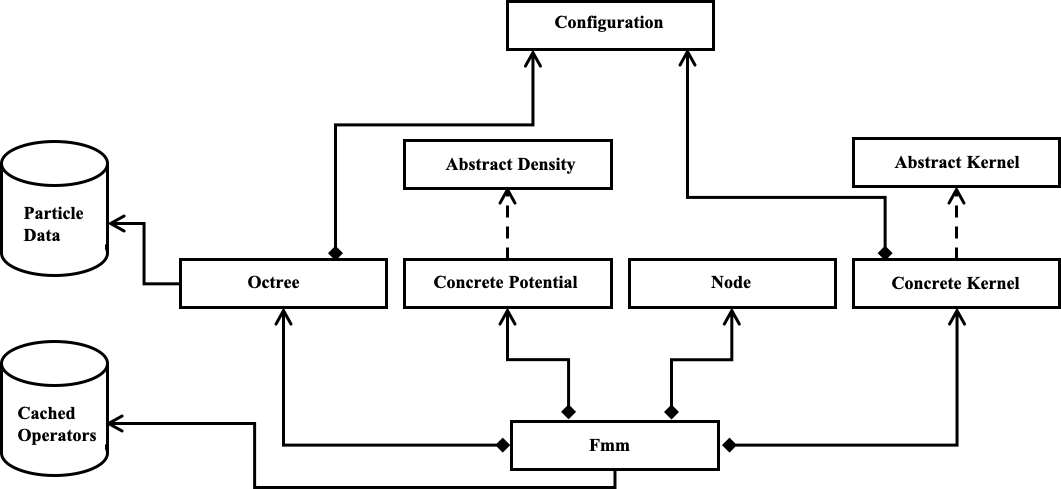
\includegraphics[width=\textwidth]{chapter2/object_organisation.png}}
    \vspace{0pt}
    \caption{Object hierarchy of \gls{PyExaFMM}. Objects are illustrated with
    square boxes, and data (either on disk, or in a cache) by a cylinder using
    standard software engineering convention \cite{Gamma:1994:Addison}. Solid
    lines indicate a dependent relationship, whereas dashed lines
    indicate an inheritance relationship. A diamond arrow head indicates an
    object instantiation, a pointed arrow head indicates the direction of a
    dependency.}
    \label{fig:2_5_architecture}
\end{figure}

\begin{figure}
    \centering
    {
\includegraphics[width=0.6\textwidth]{chapter2/kernel_strategy.png}}
    \vspace{0pt}
    \caption{Strategy design pattern implemented for the Kernel class.  Solid
    lines indicate a dependent, relationship dashed lines
    indicate an inheritance relationship. A diamond arrow head indicates an
    object instantiation, a pointed arrow head indicates the direction of a
    dependency.}
    \label{fig:2_5_strategy_kernel}
\end{figure}

The main object hierarchy used in \gls{PyExaFMM} is shown in figure
(\ref{fig:2_5_architecture}). The first major design principle followed is dependency
inversion, whereby components are arranged in a hierarchy such that downstream
components, whether they be objects or entire modules, are not dependent on
upstream components for any of their logic. Instead, they are coupled together via
abstractions in the form of known interfaces \cite{Gamma:1994:Addison}. \gls{PyExaFMM} is architected
around the main `Fmm' object, which is placed downstream, at the top of the object hierarchy.
This object contains methods that implement the logic for the
upward and downward pass steps of the \gls{FMM} loop, as well as access methods
for the source and target particle data, and the results of the expansion at each box, for each level of the associated octree.
In \gls{PyExaFMM}, a configuration object, specified via a \textbf{\gls{JSON}} file, is instantiated
at runtime. This is used to instantiate an Fmm object with its upstream dependencies.
Namely, an Octree object is configured, which creates a linear octree as well
as the \gls{JIT} compiled bitwise methods for tree traversal, from user
specified source and target particle data. Additionally, a user specified kernel choice
from the configuration file is used to instantiate a kernel object.
This kernel object is defined using the strategy design pattern
\cite{Gamma:1994:Addison}, illustrated in figure (\ref{fig:2_5_strategy_kernel}).
This pattern allows for concrete implementations of kernel objects to be separated
from the context in which they're used, allowing the user - in this case the
Fmm object - to access kernel functions via a uniform interface. Kernel
objects also allow for the encapsulation of
kernel specific information such as their scaling properties at different levels
of an octree.  This allows \gls{PyExaFMM} to be trivially extended to work with
new kernel functions, as the main loop relies only on the interface enforced by the
abstract kernel object. Furthermore, the precomputed operator matrices are loaded from a cache,
and injected into the Fmm object. Crucially, this means that the Fmm object can
remain ignorant of the implementation details of how these operators were computed.

The main point to note is that a loose hierarchy of objects allows for
the logic of the main \gls{FMM} loop to be separated from the code it depends on,
 for example for the creation and partitioning of an octree.
 Safe interactions between objects are further enforced by interfaces for data containers.
Specifically the Abstract Density and Node classes define interfaces for access to concrete Potential Density
objects (used to store the potential computed at a target particle as a result
of the FMM algorithm), and the multipole or local expansions for a given box in an octree respectively,
as well as their underlying Numpy containers, in a uniform manner.
These types of objects are often referred to as return objects in object-oriented
design as they enforce the format of the result of a computation,
here they help offer guarantees to their client, the main Fmm object,
about the dimensions and data types of their respective containers.

The second major design principle followed by \gls{PyExaFMM} is
the separation of concerns, whereby implementation details of distinct
components of a program are separated by modules, with known interfaces
\cite{Gamma:1994:Addison}. Specifically, \gls{PyExaFMM} separates into independent
scripts: the code for operator caching discussed in Section \ref{sec:2_3_operator_caching},
and the code for SVD based compression of the M2L operator matrices discussed in
Section \ref{sec:2_4_svd_compression}. These scripts are accessible via the
command-line, through a custom command-line interface, invoked with the command
prefix `ci', created as a part of \gls{PyExaFMM} package. We defer to the \gls{PyExaFMM}
documentation for more information about the command-line interface, however a
basic workflow would start at the command line, creating the \gls{M2M}
\gls{L2L} and \gls{M2L} operator matrices, and compressing the \gls{M2L} matrices,

\begin{verbatim}
Last login: <Day> <Month> <Date> 00:00:00 on console
user@Workstation ~ % ci compute-operators
user@Workstation ~ % ci compress-m2l
\end{verbatim}

These commands are again configured using the \gls{JSON} configuration file
which specifies the parameters used in a simulation, such as the order the
multipole and local expansions. Following the execution of the above,
\gls{PyExaFMM} is automatically configured with the required
operator and particle data, and simulations can be run from within a Python
interpreter or as a script using the following syntax,

\begin{python}
from fmm.fmm import Fmm

# Instantiate FMM object
fmm = Fmm(config_filename='my_custom_config.json')

# Run Upward Pass
fmm.upward_pass()

# Run Downward Pass
fmm.downward_pass()

# Get Results at Target Points
fmm.result_data
\end{python}

At runtime, the instantiation of the Fmm object is preceded by the injection of
dependencies from beneath it in the object hierarchy. However, this complexity is
hidden from the user, who only specifies simulation parameters and source
and target particle data locations via a \gls{JSON} configuration file, and interacts
with simulation outputs via the Fmm object's interface.

The utility of separating functionality to do with operator computation, and
compression into separate scripts is that it allows for iterative optimisation
without impacting on the main logic, or design, of \gls{PyExaFMM}. For example,
the main Fmm object is in general ignorant of whether multiprocessing
is being used in operator precomputations, or what the regularisation parameter
was taken to be for computing pseudoinverses of kernel operator matrices
via the SVD has been taken to be, or other specific optimisations outside of the
main loop's logic. This is as it should be, as if the Fmm
object contained too many implementation details it would obfuscate the logic,
making the code harder to debug or write unit tests for. This
encapsulates the idea of the separation of concerns.

\gls{PyExaFMM} takes this further by creating modules for specific
operations called by these scripts; specifically it offers its own multiprocessing
and SVD utility modules, which offer wrappers around common interfaces from
underlying standard Python functionality, specialised for usage in \gls{PyExaFMM}.
This offers an advantage in that their implementation can also be changed,
without effecting the logic of the operator computation and compression scripts.
For example, the planned extension to randomised \gls{SVD} methods discussed in
Section \ref{sec:2_4_svd_compression} can be separately implemented in \gls{PyExaFMM}'s
\gls{SVD} utility module while maintaining the wrapper's interface, allowing for the new
functionality to propagate into the operator compression script without
a change of the script's logic. Separation of concerns as a design
principle naturally leads to extensible code \cite{Gamma:1994:Addison}.
}


    \chapter{Experiments \& Results}\label{chpt:3}
All experiments are computed on a 2.4 GHz Quad-Core Intel Core i5 processor.
Additionally, all results are computed and stored in double precision, unless
otherwise specified.

\section{Benchmarking}\label{sec:3_1_benchmarking}
The major usage of \gls{JIT} compilation by \gls{PyExaFMM} is in the construction
of the Octree, including the calculation of the interaction lists for target
boxes, and to accelerate functions for its traversal. The impact of \gls{JIT}
compilation on tree construction is illustrated in figures
(\ref{fig:3_1_octree}) and (\ref{fig:3_1_octree2}), where octrees constructed with
Numpy and Numba together are compared to octrees constructed with just Numpy.
Each tree is constructed to a maximum depth of 5 levels over a unit box
centered at the origin. The construction time is measured against
the numbers of particles $N$ placed in the tree, which are taken to be
both the sources and the targets. The construction
is repeated five times on each problem size $N$ for statistics, though in both
figure (\ref{fig:3_1_octree}) and (\ref{fig:3_1_octree2}) the error bars, taken
from the standard deviations, are generally too small to see. Figure (\ref{fig:3_1_octree2})
illustrates how the multiplicative speedup offered by \gls{JIT} compilation via
Numba has an optimimum problem size $N$, after which the speedups provided diminish.

\begin{figure}[ht]
    \centering

  {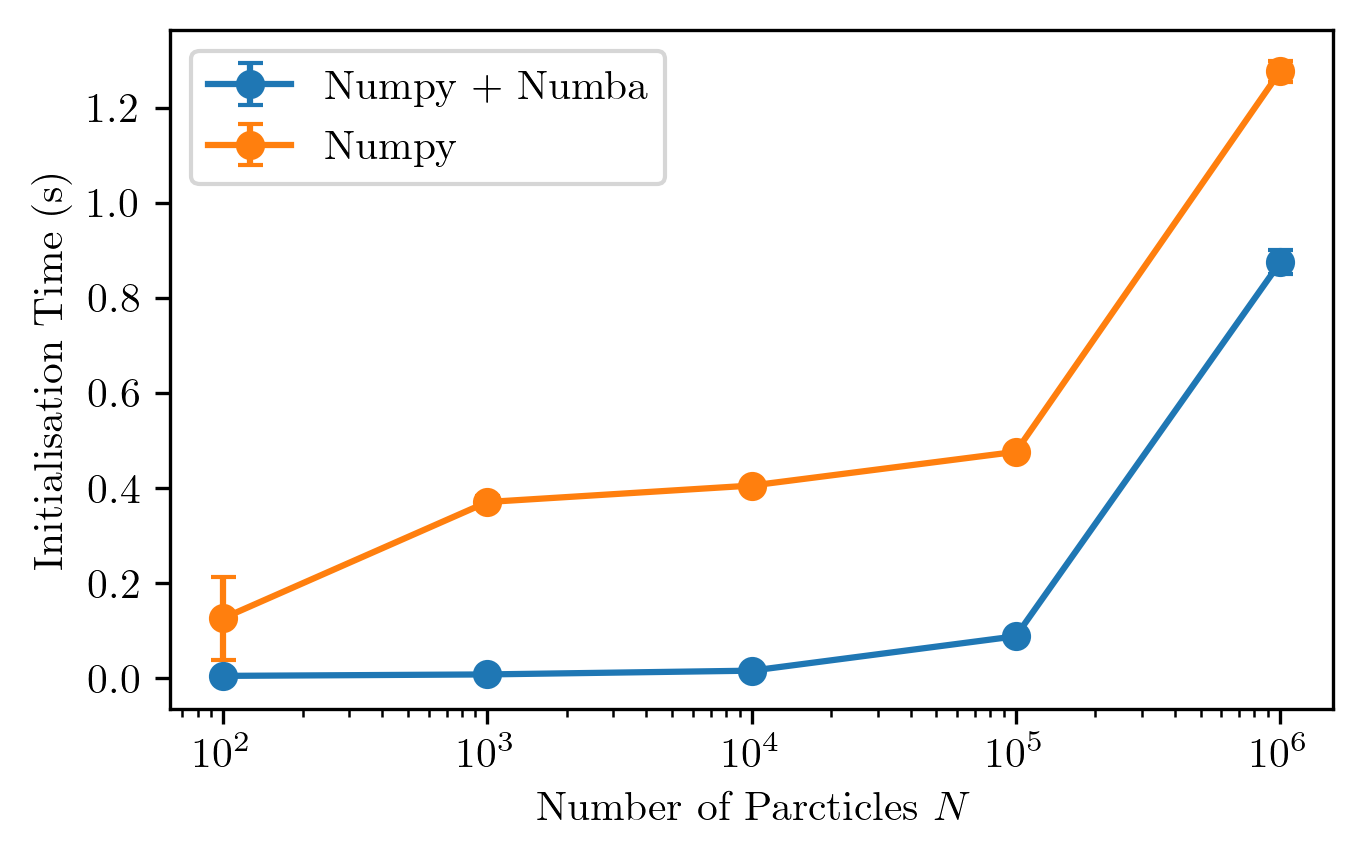
\includegraphics[width=0.9\textwidth]{chapter3/octree.png}}
  \vspace{0pt}
    \caption{
        Comparison of octree initialisation time versus number of particles $N$
        when using Numpy and Numba, to just using Numpy.
    }
    \label{fig:3_1_octree}
\end{figure}

\begin{figure}[ht]
    \centering

  {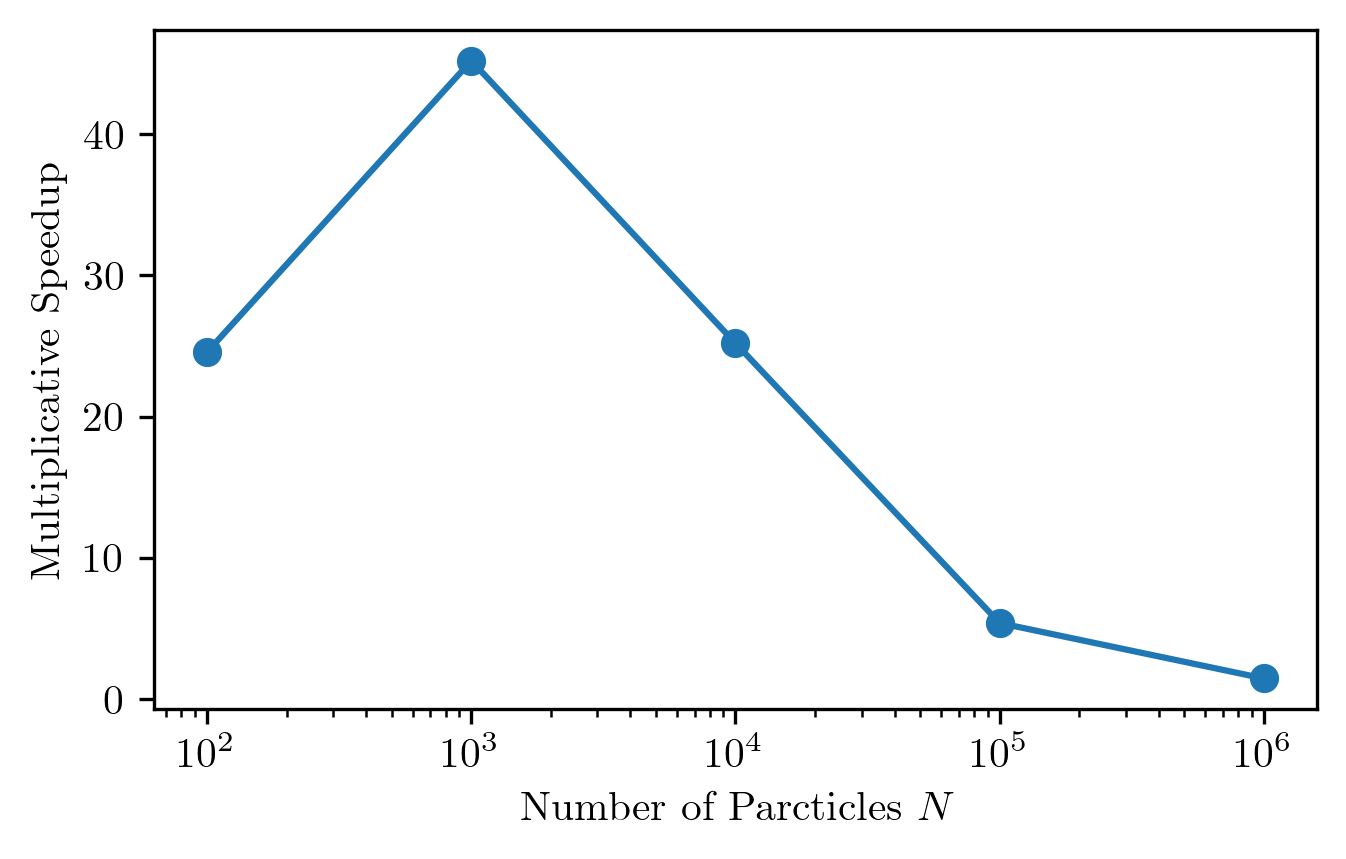
\includegraphics[width=0.9\textwidth]{chapter3/octree2.png}}
  \vspace{0pt}
    \caption{
        Multiplicative speedup offered by using Numba on top of just Numpy for
        initialising octrees.
        The analysis used to calculate the errors is provided in
        Appendix \ref{app:errors}, Section \ref{sec:app_numba}.
    }
    \label{fig:3_1_octree2}
\end{figure}

Table (\ref{table:3_1_jit}) provides timing comparisons for all the octree traversal
functions used in \gls{PyExaFMM} when using Numba and Numpy, or just Numpy alone.
\gls{JIT} compilation relies on a preliminary code analysis, to find optimisations
in the interpreted byte code, this can lead to relatively longer runtimes when
a \gls{JIT} compiled function is first invoked, in comparison to subsequent
invocations. All the calculations in table (\ref{table:3_1_jit}) were run for a
Morton key of 100 placed in a unit box centered at the origin, and were repeated
one hundred times for statistics. We observe that the preliminary analysis step for
some \gls{JIT} compiled function is so expensive that the mean time for the \gls{JIT}
compiled function is significantly longer than using a function with Numpy alone.
Further investigation is needed to understand exactly why the \gls{JIT} preliminary
analysis takes so much longer for some Numpy based functions than others.

\begin{table}[ht]
    \centering % used for centering table
    \begin{tabular}{c c c} % centered columns (4 columns)
    \hline\hline %inserts double horizontal lines
    Method & Numpy + Numba & Numpy \\ [0.5ex] % inserts table
    %heading
    \hline % inserts single horizontal line
    Get Level of a Key & 280 ns ± 276 ns  & 1.01 µs ± 265 ns \\ % inserting body of the table
    Get Offset of Key & 29.6 µs ± 291 µs & 804 ns ± 324 ns \\
    Remove Offset from a Key & 30.7 µs ± 301 µs & 1.83 µs ± 566 ns \\
    Get Octant of a Key & 23.6 µs ± 231 µs & 2.16 µs ± 2.71 µs \\
    Get Octant Index From Key & 64.4 µs ± 632 µs & 10.7 µs ± 3.82 µs \\
    Get Key From Octant Index & 36.4 µs ± 356 µs & 11.1 µs ± 3.54 µs \\
    Get Octant Index From Cartesian Coordinate & 50.4 µs ± 484 µs & 17.3 µs ± 21 µs \\
    Get Key From Cartesian Coordinate & 2.71 µs ± 1.58 µs & 30.4 µs ± 20.3 µs \\
    Get Box Center From Octant Index & 49.2 µs ± 476 µs & 21.7 µs ± 27.2 µs \\
    Get Box Center From Key & 60.5 µs ± 581 µs & 22.4 µs ± 7.52 µs \\
    Get Parent Key & 29.7 µs ± 292 µs & 2.47 µs ± 546 ns \\
    Get Child Keys & 37.6 µs ± 361 µs & 8.62 µs ± 11.2 µs \\
    Get All Neighbor Keys & 98.4 µs ± 803 µs & 445 µs ± 80.1 µs\\
    Get All Possible Keys In Interaction List & 98.4 µs ± 803 µs & 1.67 ms ± 225 µs \\ [1ex] % [1ex] adds vertical space
    \hline %inserts single line
    \end{tabular}
    \label{table:3_1_jit} % is used to refer this table in the text
    \caption{
        Benchmarking tree traversal functions implemented in \gls{PyExaFMM} by
        comparing Numpy functions \gls{JIT} compiled with Numba, to plain Numpy functions.
        Errors are taken from the standard deviation over trials. Results and
        errors are truncated to 3 significant figures.
        } % title of Table
\end{table}


The loading and saving speeds of files into/from memory, as a function of file size,
using HDF5 in comparison to Python's native object serialisation library, Pickle,
are illustrated in figures (\ref{fig:3_1_loadtime}) and (\ref{fig:3_1_savetime})
respectively. Each trial was repeated five times with each file size for statistics.
The multiplicative speedups for loading and saving using HDF5 are illustrated
in figures (\ref{fig:3_1_loadtime_speedup}) and (\ref{fig:3_1_savetime_speedup})
respectively.

We observe that the speedup offered by HDF5 for loading and saving
data is approximately constant over file size. The reasons for this are due to the underlying
techniques used by each method. Roughly speaking, HDF5 stores raw numeric data
alongside a header file describing its dimensions, as a contiguous byte stream
on disk which allows for optimised methods to quickly search and retrieve data
\cite{collette2013python}. Object serialisation is designed to work with arbitrary
Python objects, raw numeric data is not stored, rather it is first compressed
into an intermediate representation, that results in a byte stream which is then
stored on disk. This data is stored alongside the metadata for the object, such
as it's initialisation code, and even any dependent objects it may have. The
intermediate representation allows any objects to be serialised in the same
manner \cite{pickle}.

\begin{figure}
    \centering

  {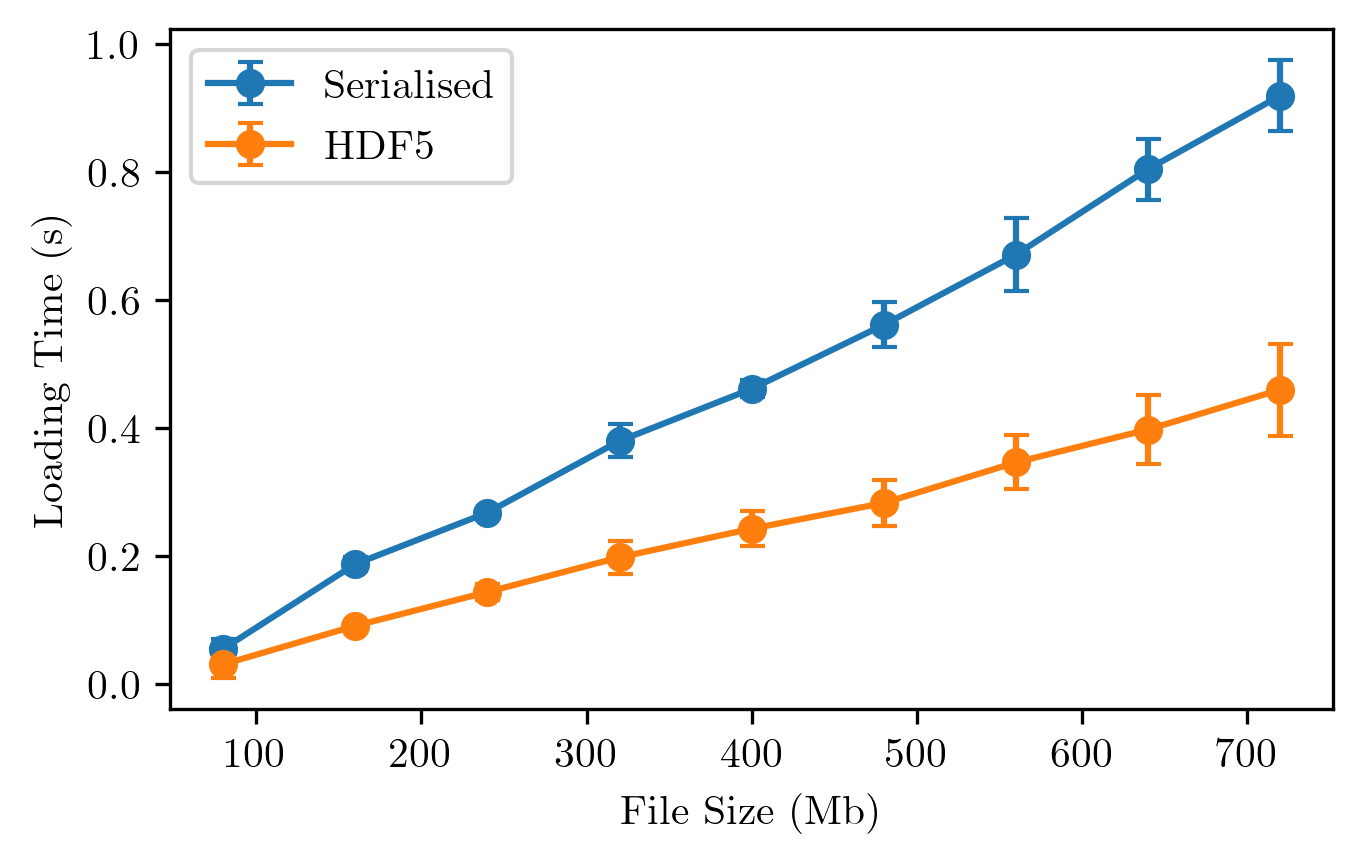
\includegraphics[width=0.9\textwidth]{chapter3/loadtime.png}}
  \vspace{0pt}
    \caption{
        Loading times versus File Size comparing object serialisation to HDF5.
    }
    \label{fig:3_1_loadtime}
\end{figure}


\begin{figure}
    \centering

  {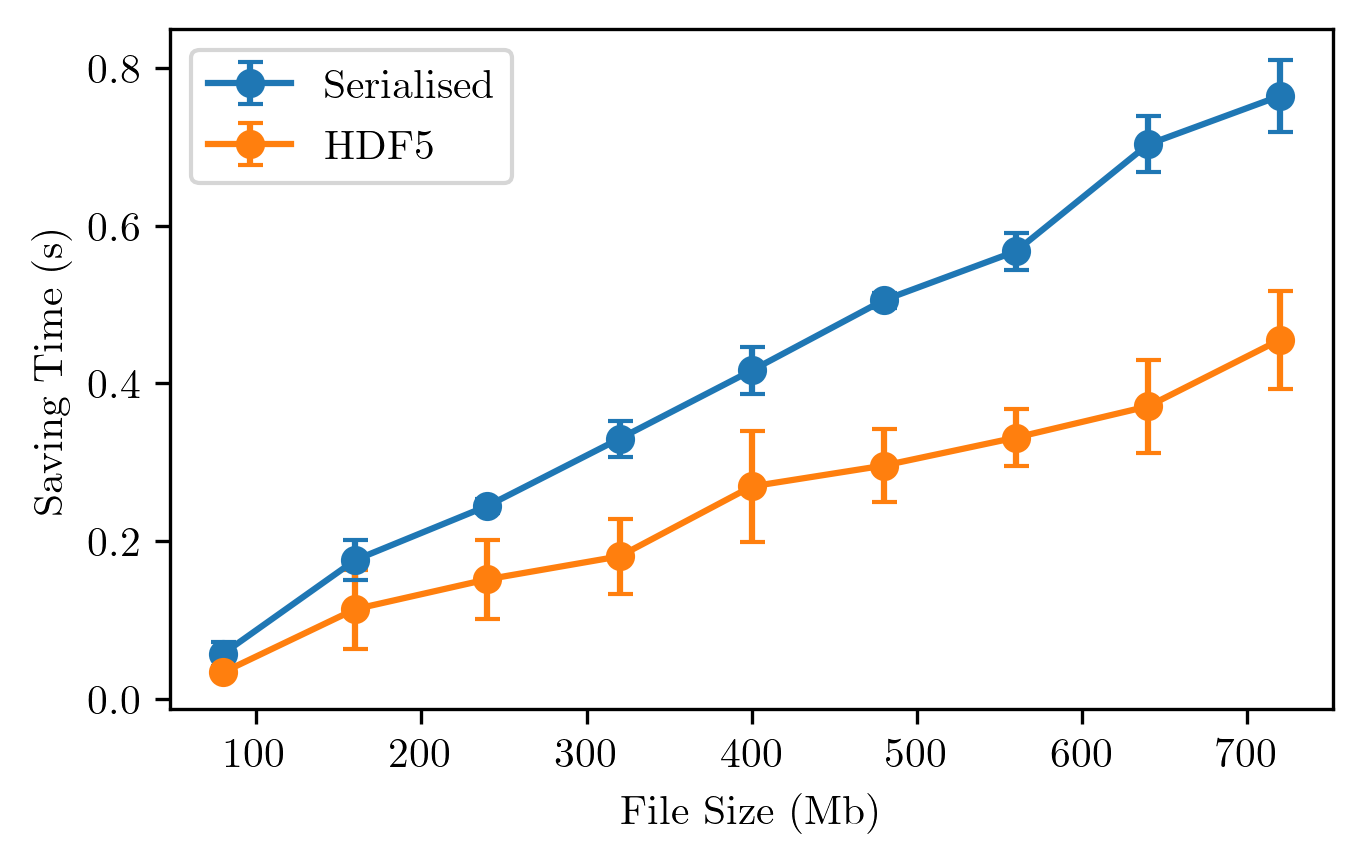
\includegraphics[width=0.9\textwidth]{chapter3/savetime.png}}
  \vspace{0pt}
    \caption{
        Saving times versus File Size comparing object serialisation to HDF5.
    }
    \label{fig:3_1_savetime}
\end{figure}


\begin{figure}
    \centering

  {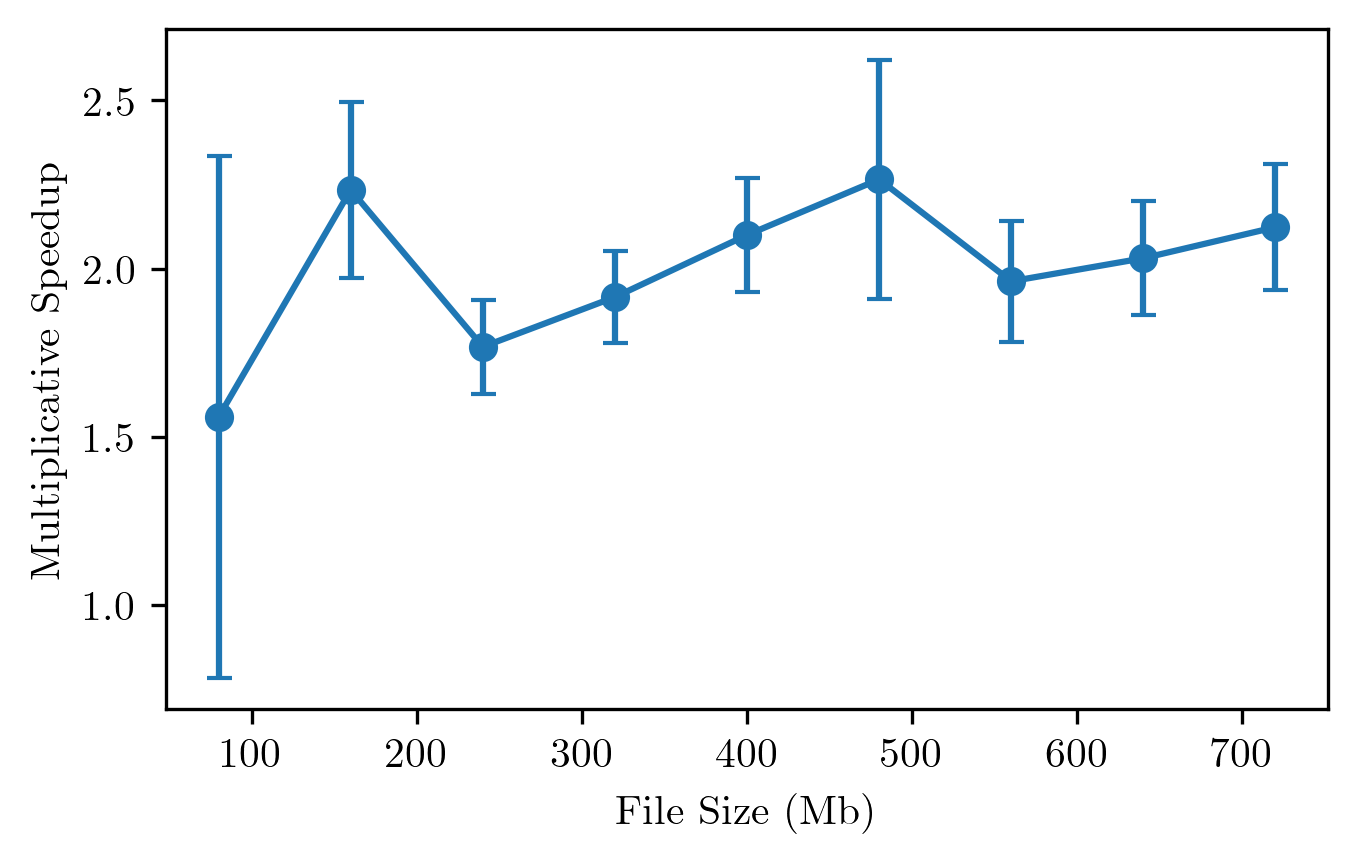
\includegraphics[width=0.9\textwidth]{chapter3/loadtime_speedup.png}}
  \vspace{0pt}
    \caption{
        The multiplicative speedup offered by HDF5 over object serialisation
        as a function of file size for loading files.
        The analysis used to calculate the errors is provided in
        Appendix \ref{app:errors}, Section \ref{sec:app_numba}.
    }
    \label{fig:3_1_loadtime_speedup}
\end{figure}


\begin{figure}
    \centering

  {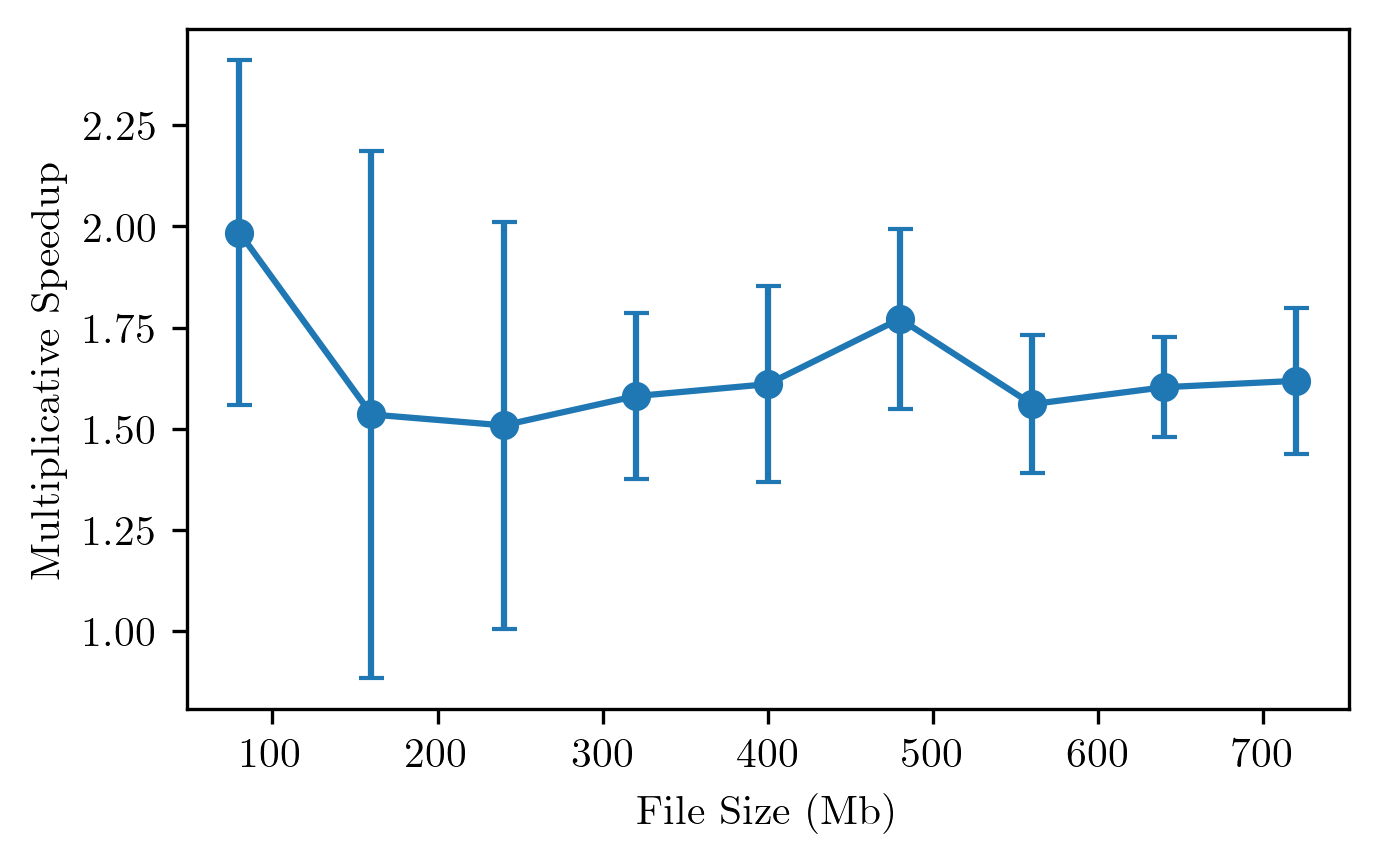
\includegraphics[width=0.9\textwidth]{chapter3/savetime_speedup.png}}
  \vspace{0pt}
    \caption{
        The multiplicative speedup offered by HDF5 over object serialisation
        as a function of file size for saving files.
        The analysis used to calculate the errors is provided in
        Appendix \ref{app:errors}, Section \ref{sec:app_numba}.
    }
    \label{fig:3_1_savetime_speedup}
\end{figure}


The effect of multiprocessing on time to calculate the operator matrix precomputations is
illustrated in figure (\ref{fig:3_1_multiproc}). Here we solve
for the operator matrices of the model electrostatic problem in three dimensions
(\ref{eq:electrostatic_paradigm}) for a 1000 randomly distributed particles placed in
a unit cube. These are taken to be both sources and targets, with unit charges
placed on all sources. The problem is discretised using an octree with a maximum depth of 3 levels,
and we vary the number of processor cores accessible to the script.
Relevant surfaces are calculated to order $p=2$, and therefore discretised
with 8 quadrature points (\ref{eq:2_2_quadrature_points}). The parameters for
the relative sizes of different surfaces are the same as those provided
in Chapter \ref{chpt:2_strategy_for_practical_implementation},
Section \ref{sec:2_3_operator_caching}. The speedup offered by increasing the
number of processor cores is non-linear, this is indicative of a communication
overhead, and the fact that multiprocessing has been implemented to a very
basic degree with the required data being copied to each process, even if very large.

\begin{figure}[ht]
    \centering

  {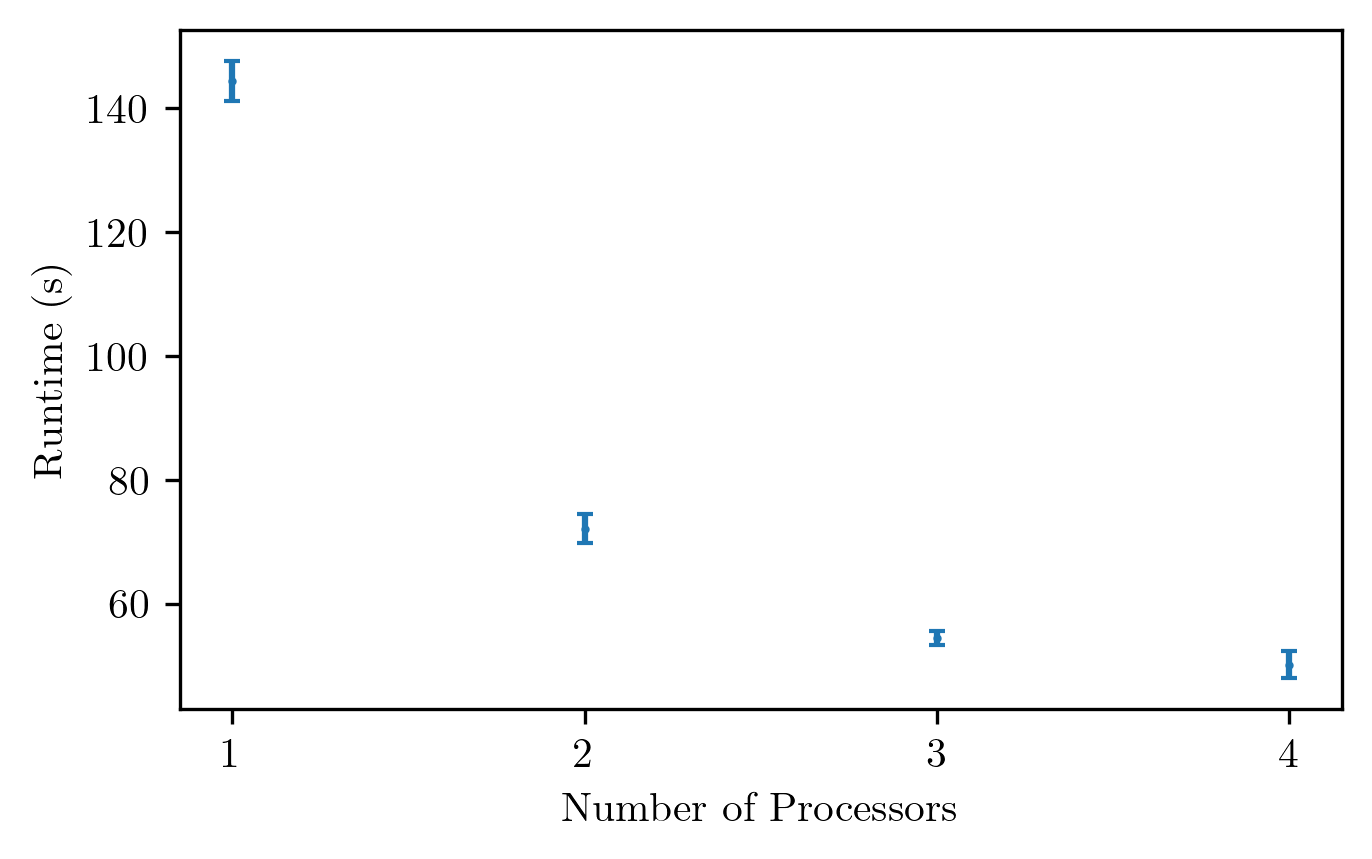
\includegraphics[width=0.9\textwidth]{chapter3/multiproc.png}}
  \vspace{0pt}
    \caption{Runtime versus number of processors used for operator precomputations
    for the model problem (\ref{eq:electrostatic_paradigm}). Error bars are
    plotted using standard deviation.
    }
    \label{fig:3_1_multiproc}
\end{figure}

We benchmark the asymptotic run time of \gls{PyExaFMM} in comparison to direct computation in figure
(\ref{fig:3_1_complexity}), with same octree parameters as used for benchmarking
the operator precomputation, but with an increasing number of target and source
particles $N$ for our model problem (\ref{eq:electrostatic_paradigm}). The
calculations are run three times for each problem size for statistics.
Assuming a power relationship between run time $t$ and problem size $N$,

\begin{equation}
    t = N^x,
\end{equation}

where $x$ is unknown, taking logarithms allows one to apply least squares fitting
to fit a linear relationship to,

\begin{equation}
    \log(t) = x \log(N),
\end{equation}

computing the value of $x$ from the gradient. Performing this calculation for the
results from \gls{PyExaFMM} and direct calculation we report $x=1.14$ (2 d.p) for
\gls{PyExaFMM}, and $x=1.98$ (2 d.p) for the direct computation. This implies an approximate
asymptotic complexity of $O(N)$, and $O(N^2)$ for \gls{PyExaFMM} and direct methods
respectively in line with what is expected, with the limitation that this has
been tested on relatively small inputs of only $O(10^3)$ particles.

\begin{figure}[ht]
    \centering

  {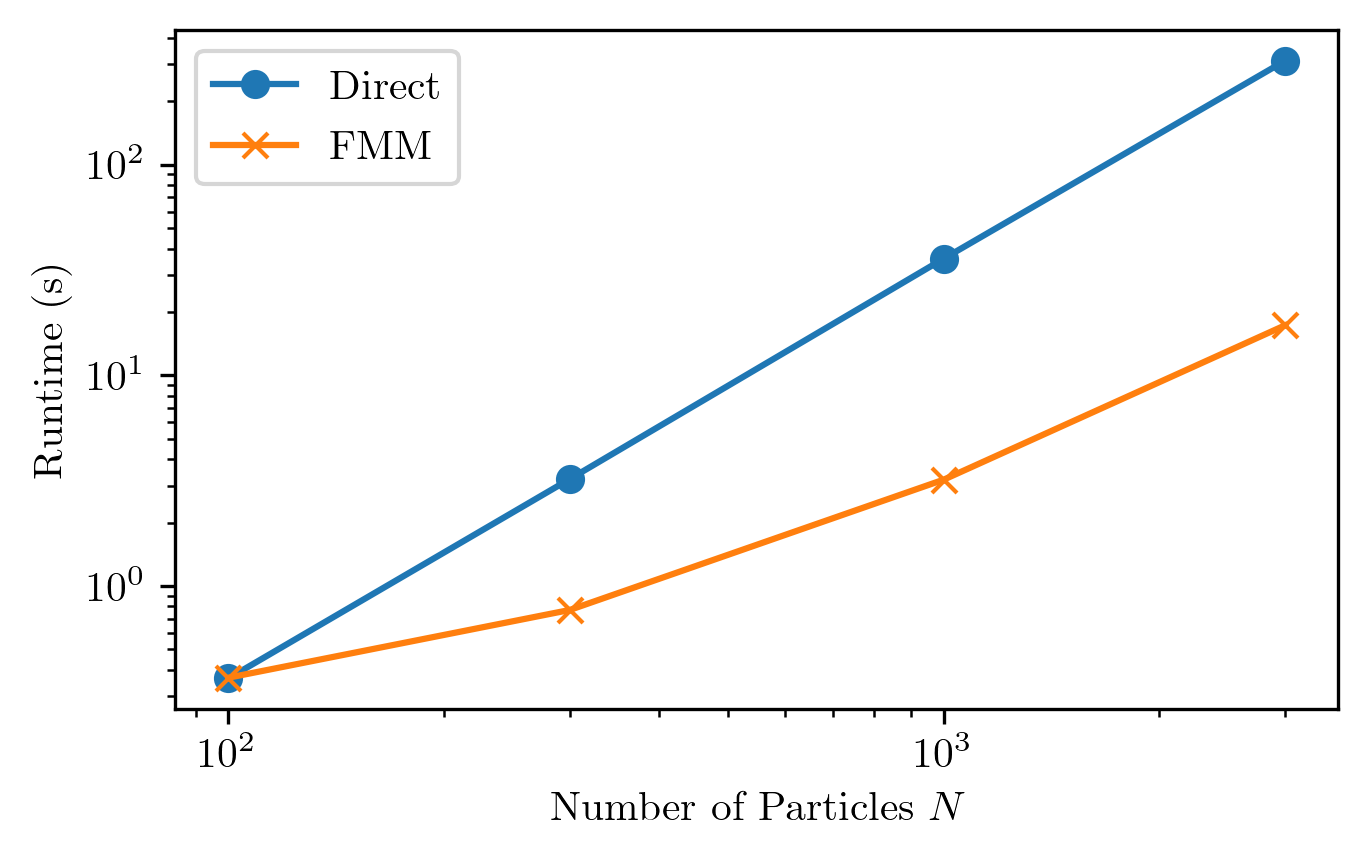
\includegraphics[width=0.9\textwidth]{chapter3/complexity.png}}
  \vspace{0pt}
    \caption{
        Runtime versus problem size to solve the model problem
        (\ref{eq:electrostatic_paradigm}) using direct calculations and
        \gls{PyExaFMM}.
    }
    \label{fig:3_1_complexity}
\end{figure}

We report that a simulation with the above octree and
$N=3000$ takes $17.1 \pm 0.2$ s, over the three runs with
error calculated from standard deviation and reported to 1 s.f. From correspondence
with the authors of ExaFMM-T, we can report their corresponding benchmark figure,
calculated on a 14 Core Intel i9-7940X \gls{CPU} with $N=10^6$ particles
randomly distributed in a unit cube, it takes 0.52 s to perform a $p=4$ degree
computation, including tree construction but excluding the
operator precomputations, in single precision \cite{exafmm}. Time limitations for this project
makes it difficult to perform comparisons using equivalent hardware, however
disparities in hardware are unlikely to explain the magnitude of superiority
of ExaFMM-t's performance in comparison to \gls{PyExaFMM}.

ExaFMM-T implements a range of optimisations which represent future avenues
of software development for \gls{PyExaFMM}. Specifically, they distribute the
\gls{P2P} and \gls{M2L} operations on \gls{GPU}s, as discussed in Chapter
\ref{chpt:2_strategy_for_practical_implementation},
Section \ref{sec:2_3_operator_caching}, as well as using \gls{OpenMP} to share
precomputed surfaces across processes in the operator precomputations.
\gls{PyExaFMM} does not distribute any calculations on \gls{GPU}s, and
wastefully copies surface data to each process for the operator precomputations.
Furthermore, ExaFMM-t optimises the application of the kernel function,
firstly by the inverse operation in (\ref{eq:electrostatic_paradigm}) using a Newton
iteration to approximate $x = 0.5x(w-ax^2)$ to approximate $x \approx a ^{-1/2}$,
the computation for which highly-optimised implementations exist
\cite{Lomont:2003, sqrt}. Secondly \textbf{\gls{AVX}} vectorisation is used
to apply the kernel function. Roughly speaking, \gls{AVX} vectorisation allows
for parallel execution of \gls{SIMD} type instructions in a \gls{CPU}. With similar
optimisations, PVFMM is able to report a 3.8 times multiplicative speed up, in
comparison to naive applications of the Laplace kernel \cite{Malhotra:2015:CCP}.


\section{Optimum Target Rank}\label{sec:3_2_svd_params}

\begin{figure}[ht]
    \centering

  {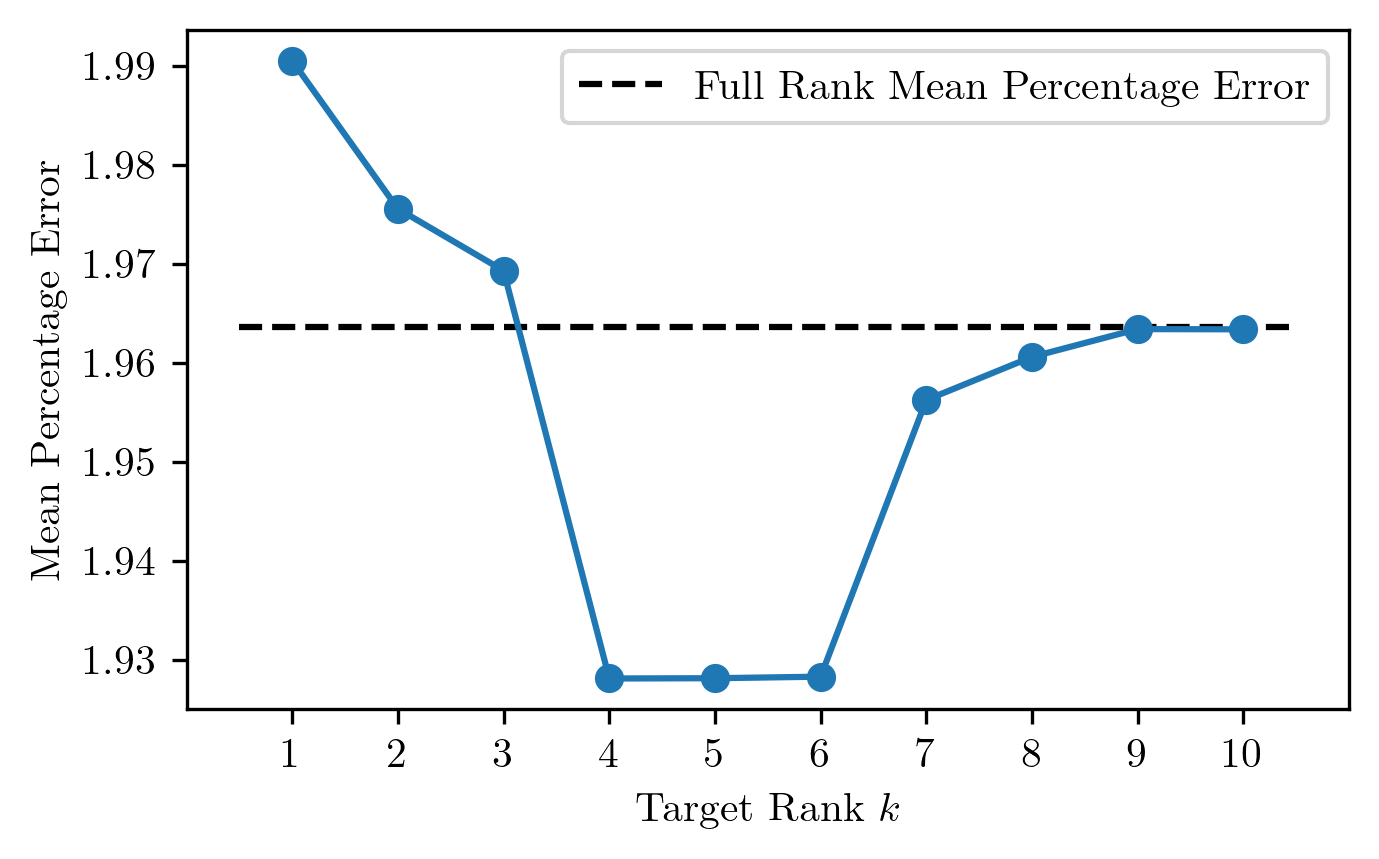
\includegraphics[width=0.9\textwidth]{chapter3/svd.png}}
  \vspace{0pt}
    \caption{Foo Bar}
    \label{fig:3_2_svd}
\end{figure}

    \chapter{Conclusion}
\section{Section 1}
\lipsum[2-4]

    \appendix
    \chapter{Appendix}
\section{FMM Algorithm Specification}
\label{app:analytic_fmm}

This pseudo-code is adapted from \cite{Greengard:1987:Yale}.

\hfill


\textbf{Initialisation}: Choose a level of refinement of $n \approx \log_8 N$
and precision $\epsilon$, set $p= \lceil -\log_2(\epsilon) \rceil$\footnote{
    Different authors have different suggestions for $p$, the authors
    of \cite{Ying:2004:JCP} use $p = \log_c \epsilon$ with $c=\frac{4-\sqrt{3}}{\sqrt{3}}$
}. \\

\textbf{Upward Pass}
\begin{center}
    \textbf{Step 1}
\end{center}
Form multipole expansions of potential field due to particles in each box at
leaf level. \\

\noindent \textbf{do} $\textit{ibox}=1,..,8^l$ \\
\indent   Form $p^{th}$ degree multipole expansion for each leaf box.\\
\noindent \textbf{end}

\begin{center}
    \textbf{Step 2}
\end{center}

Translate Multipole expansion to coarser levels from the bottom up.\\

\noindent \textbf{do} $l=n-1,..,0$ \\
\indent \textbf{do} $\textit{ibox}=1,..,8^n$ \\
\indent \indent Perform M2M operations. \\
\indent \textbf{end} \\
\noindent \textbf{end} \\

\textbf{Downward Pass} \\

Computations at the coarsest possible level. For a given box, done by including
interactions with those boxes which are \gls{well-separated}, and whose interactions
have not been accounted for at the parent level.

\begin{center}
    \textbf{Step 3}
\end{center}

Form local expansion about center of each box at each level $l \leq n-1$, describes
field due to all particles that are not contained in the current box, it's \gls{near-neighbours}
or it's secondary near neighbors.

\noindent \textbf{do} $l=1,...,n-1$ \\
\indent \textbf{do} $\textit{ibox}=1,...,8^l$ \\
\indent \indent Perform M2L translations. \\
\indent \textbf{end} \\
\indent \textbf{do} $1,...,8^l$ \\
\indent \indent Perform L2L operations.\\
\indent \textbf{end} \\
\noindent \textbf{end}\\

\begin{center}
    \textbf{Step 4}
\end{center}

After this step, local expansions are available at the leaf level. One can use
this to evaluate potential at leaves from all particles in the far field.\\

\noindent \textbf{do} $\textit{ibox}=1,...,8^n$ \\
\indent Find local expansion at leaf level, by doing M2L from interaction list. \\
\noindent \textbf{end}

\begin{center}
    \textbf{Step 5}
\end{center}
Evaluate local expansions at particle positions in all leaves\\

\noindent \textbf{do} $\textit{ibox}=1,...,8^n$ \\
\indent For every particle in $\textit{ibox}$'th box, evaluate local expansion. \\
\noindent \textbf{end} \\

\begin{center}
    \textbf{Step 6}
\end{center}
Compute nearest neighbors directly,

\noindent \textbf{do} $\textit{ibox}=1,...,8^n$ \\
\indent For every particle in $\textit{ibox}$'th box, compute potential directly with nearest neighbors. \\
\noindent \textbf{end} \\


\begin{center}
    \textbf{Step 7}
\end{center}

\noindent \textbf{do} $\textit{ibox}=1,...,8^n$ \\
\indent Add direct and far field terms together for every particle in the $\textit{ibox}$\\
\noindent \textbf{end} \\


    \printglossary

    \printbibliography[heading=bibintoc]


\end{document}
